\graphicspath{{Figures/}}

\title{\fontsize{33}{45}{\huge Pattern Classification (EET 3035)\newline \vspace{8pt} \Large Lecture 05\vspace{-1.1cm}}}
\author{\vspace{-0.4cm}\\\normalsize{\bf Dr. Kundan Kumar}\\ PhD (IIT Kharagpur)\\
Associate Professor\\Department of ECE}
% - Give the names in the same order as the appear in the paper.
% - Use the \inst{?} command only if the authors have different
%   affiliation.

\institute[Indian Institute of Technology Kharagpur] % (optional, but mostly needed)
{
\includegraphics[height=.17\textheight]{SOAlogo.png}\\
 Faculty of Engineering (ITER)\\ S`O'A Deemed to be University, Bhubaneswar, India-751030\\
 \copyright\  2019 Kundan Kumar, All Rights Reserved\\
  \vspace{-1.1cm}}
% - Use the \inst command only if there are several affiliations.
% - Keep it simple, no one is interested in your street address.
\date{}
% To remove page number from a perticular slide
{
\setbeamertemplate{logo}{}
\makeatletter
\setbeamertemplate{footline}{
        \leavevmode%
  
  % First line.
  \hbox{%
  \begin{beamercolorbox}[wd=.2\paperwidth,ht=\beamer@decolines@lineup,dp=0pt]{}%
  \end{beamercolorbox}%
  \begin{beamercolorbox}[wd=.8\paperwidth,ht=\beamer@decolines@lineup,dp=0pt]{lineup}%
  \end{beamercolorbox}%
  } %
  % Second line.
  \hbox{%
  \begin{beamercolorbox}[wd=\paperwidth,ht=\beamer@decolines@linemid,dp=0pt]{linemid}%
  \end{beamercolorbox}%
  } %
  % Third line.
  \hbox{%
  \begin{beamercolorbox}[wd=.1\paperwidth,ht=\beamer@decolines@linebottom,dp=0pt]{}%
  \end{beamercolorbox}%
  \begin{beamercolorbox}[wd=.9\paperwidth,ht=\beamer@decolines@linebottom,dp=0pt]{linebottom}%
  \end{beamercolorbox}%
  }%
        }
\makeatother
\begin{frame}
\titlepage
\end{frame}
}

\section{Dimensionality Problem}
\subsection{}

\begin{frame}{Topics to be covered}
\begin{itemize}
\item Dimensionality Problem
\item Dimensionality/Feature reduction
\begin{itemize}
\item Principal component analysis
\item Linear discriminant analysis
\begin{itemize}
\item Fisher Linear discriminant
\item Multiple Discriminant Analysis
\end{itemize}
\end{itemize}
\item Feature Selection
\end{itemize}
\end{frame}


\begin{frame}{}
\begin{variableblock}{\centering \Large \textbf{\vspace{4pt}\newline Dimensionality Problem\vspace{4pt}}}{bg=slidecolor,fg=white}{bg=slidecolor,fg=white}
\end{variableblock}
\end{frame}


 
\begin{frame}{Introduction}
\begin{itemize}
\item In practical multicategory applications, it is not unusual to encounter problems involving tens or hundreds of features.
\item Intuitively, it may seem that each feature is useful for at least some of the discriminations.
\item In general, if the performance obtained with a given set of features is inadequate, it is natural to consider adding new features.
\item Even though increasing the number of features increases
the complexity of the classifier, it may be acceptable for an
improved performance.
\end{itemize}
\end{frame}

\begin{frame}{Introduction}
\begin{figure}
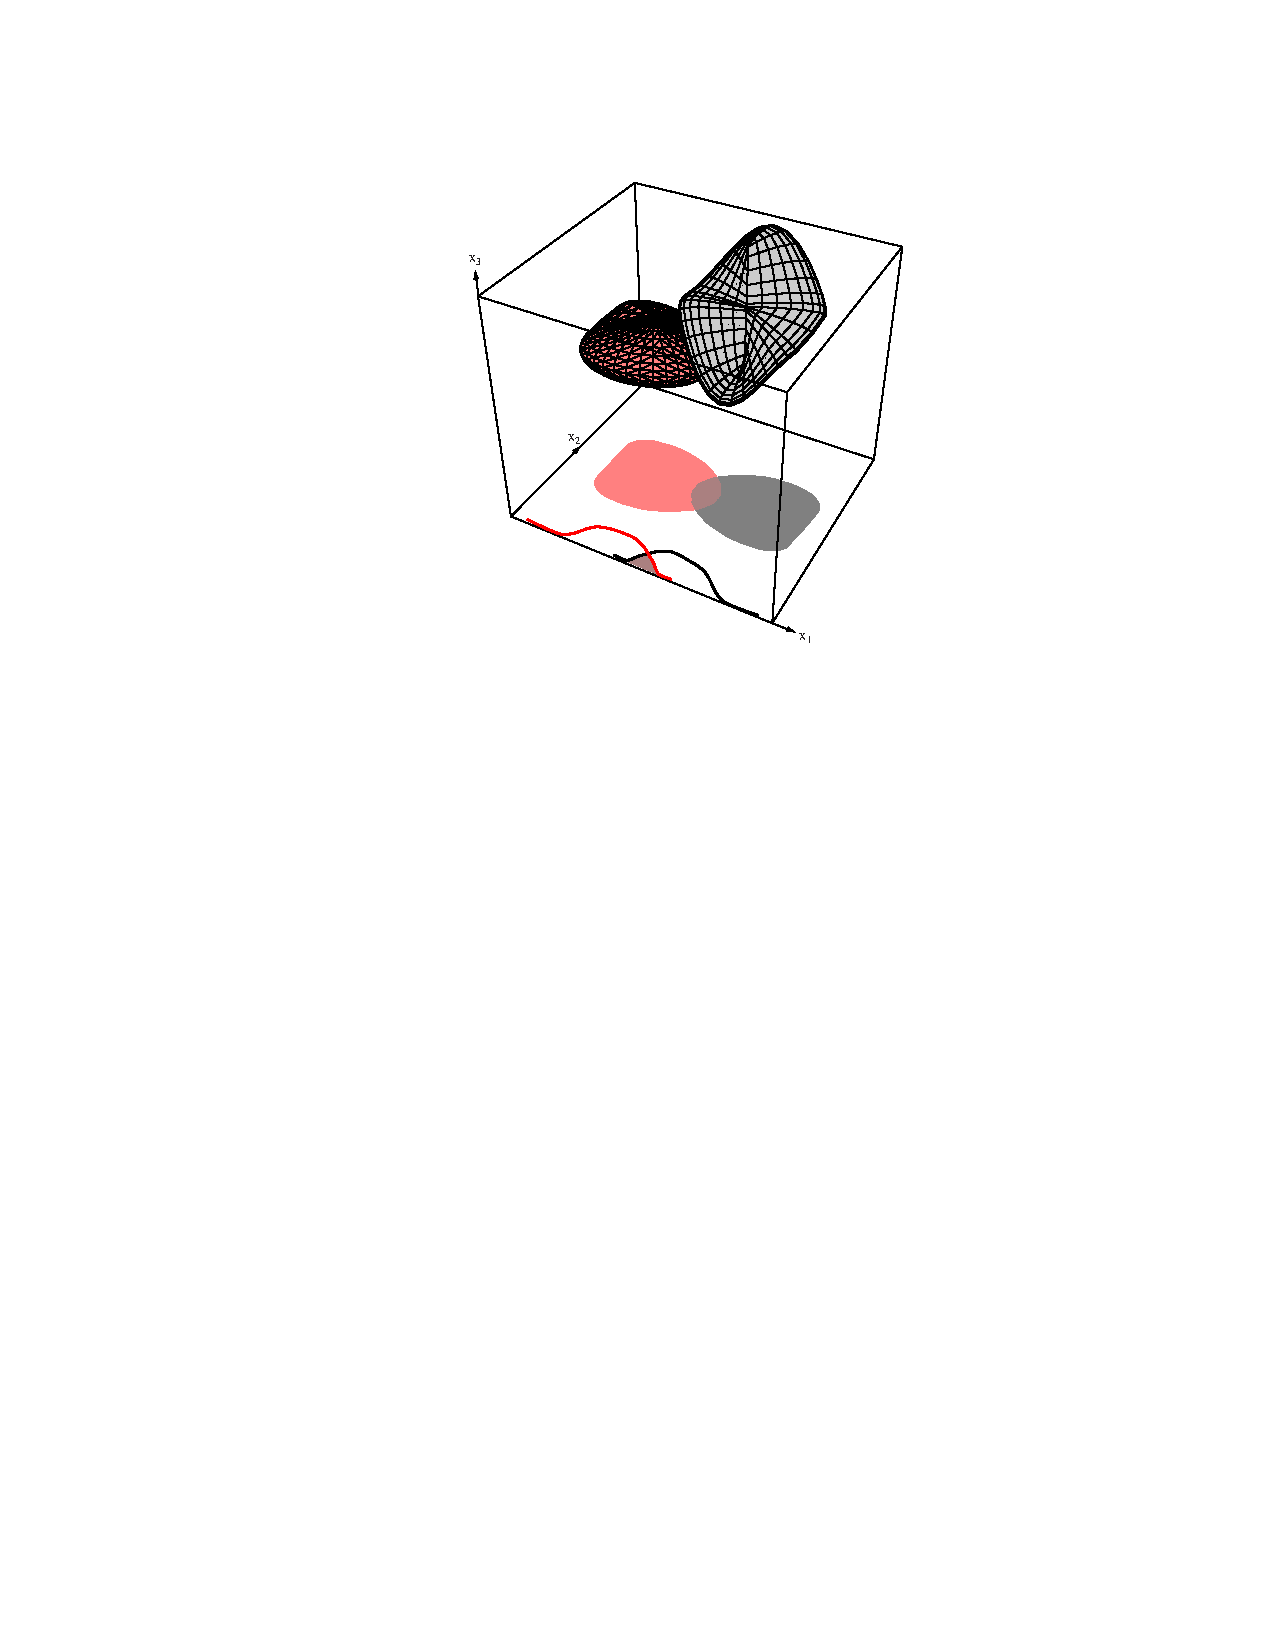
\includegraphics[scale=0.65]{DimProb01}
\caption{There is a non-zero Bayes error in the one-dimensional $x_1$ space or the two-dimensional $x_1,x_2$ space. However, the Bayes error vanishes in the $x_1,x_2,x_3$ space because of non-overlapping densities.} 
\end{figure}
\end{frame}

\begin{frame}{Problems of Dimensionality}
\begin{itemize}
\setlength{\itemsep}{12pt}
\item Unfortunately, it has frequently been observed in practice
that, beyond a certain point, adding new features leads to
worse rather than better performance.
\item This is called the \textit{\color{mycolor2}curse of dimensionality}.
\item There are two issues that we must be careful about:
\begin{itemize}
\item How is the classification accuracy affected by the
dimensionality (relative to the amount of training data)?
\item How is the complexity of the classifier affected by the
dimensionality?
\end{itemize}
\end{itemize}
\end{frame}

\begin{frame}{Problems of Dimensionality}
\begin{itemize}
\setlength{\itemsep}{12pt}
\item Potential reasons for increase in error include
\begin{itemize}
\item wrong assumptions in model selection,
\item estimation errors due to the finite number of training samples for high-dimensional observations (overfitting).
\end{itemize}
\item Potential solutions include
\begin{itemize}
\item reducing the dimensionality,
\item simplifying the estimation.
\end{itemize}
\end{itemize}
\end{frame}

\begin{frame}{Problems of Dimensionality}
\begin{itemize}
\item Dimensionality can be reduced by
\begin{itemize}
\item redesigning the features,
\item selecting an appropriate subset among the existing features,
\item combining existing features.
\end{itemize}
\item Estimation errors can be simplified by
\begin{itemize}
\item assuming equal covariance for all classes (for the Gaussian
case),
\item using regularization,
\item using prior information and a Bayes estimate,
\item using heuristics such as conditional independence,
\item $\cdots$.
\end{itemize}
\end{itemize}
\end{frame}

\begin{frame}{Problem of Dimensionality}
\begin{figure}
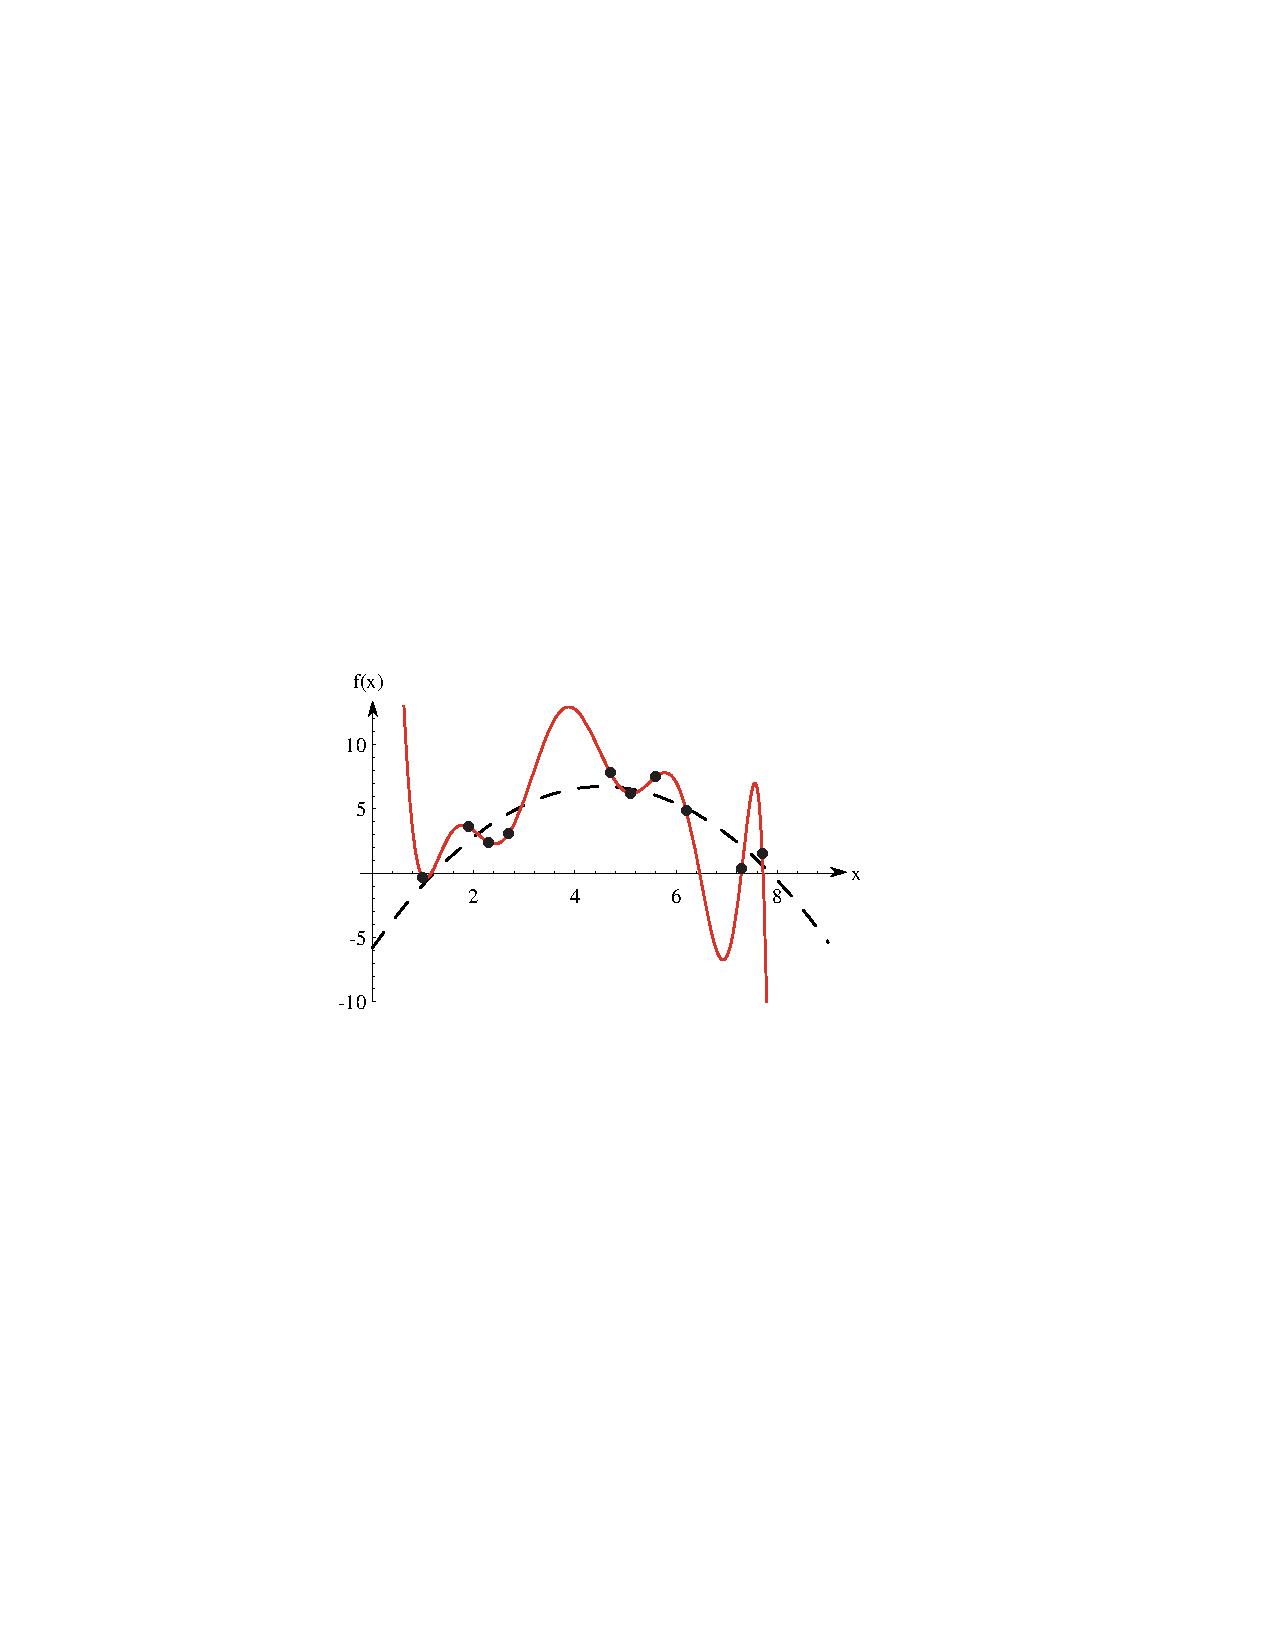
\includegraphics[scale=0.75]{DimProb02}
\caption{The ``training data'' (black dots) were selected from a quadratic function plus Gaussian noise, i.e, $f(x)=ax^2+bx+c+\varepsilon$ where $p(\varepsilon)\approx N(0,\sigma^2)$. The 10th degree polynomial shown fits the data perfectly, but we desire instead the second-order function $f(x)$, since it would lead to better predictions for few samples.}
\end{figure}
\end{frame}

\begin{frame}{Problem of Dimensionality}
\begin{itemize}
\setlength{\itemsep}{12pt}
\item All of the commonly used classifiers can suffer from the
curse of dimensionality.
\item While an exact relationship between the probability of error,
the number of training samples, the number of features, and
the number of parameters is very difficult to establish, some
guidelines have been suggested.
\item It is generally accepted that using at least ten times as
many training samples per class as the number of features
($n/d > 10$) is a good practice.
\end{itemize}
\end{frame}

\section{Component Analysis}
\subsection{}
\begin{frame}{}
\begin{variableblock}{\centering \Large \textbf{\vspace{4pt}\newline Dimensionality Reduction\vspace{4pt}}}{bg=slidecolor,fg=white}{bg=slidecolor,fg=white}
\end{variableblock}
\end{frame}

\begin{frame}{Component Analysis and Discriminants}
\begin{itemize}
\item One way of coping with the problem of high dimensionality
is to reduce the dimensionality by combining features.
\item Issues in feature reduction:
\begin{itemize}
\item Linear vs. non-linear transformations.
\item Use of class labels or not (depends on the availability of
training data).
%\item Training objective:
%\begin{itemize}
%\item minimizing classification error (discriminative training),
%\item minimizing reconstruction error (PCA),
%\item maximizing class separability (LDA),
%\end{itemize}
\end{itemize}
\item Linear combinations are particularly attractive because they
are simple to compute and are analytically tractable.
\item Linear methods project the high-dimensional data onto a
lower dimensional space.
\item Advantages of these projections include
\begin{itemize}
\item reduced complexity in estimation and classification,
\item ability to visually examine the multivariate data in two or three dimensions.
\end{itemize}
\end{itemize}
\end{frame}

%\begin{frame}{Component Analysis and Discriminants}
%\begin{itemize}
%\item Linear combinations are particularly attractive because they
%are simple to compute and are analytically tractable.
%\item Linear methods project the high-dimensional data onto a
%lower dimensional space.
%\item Advantages of these projections include
%\begin{itemize}
%\item reduced complexity in estimation and classification,
%\item ability to visually examine the multivariate data in two or three dimensions.
%\end{itemize}
%\end{itemize}
%\end{frame}

\begin{frame}{Component Analysis and Discriminants}
\begin{itemize}
\setlength{\itemsep}{12pt}
\item Given ${\rm x}\in \mathbb{R}^d$, the goal is to find a linear transformation ${\rm A}$ that gives ${\rm y} = {\rm A}^T{\rm x} \in \mathbb{R}^{d_0}$ where $d_0 < d$.
\item Two classical approaches for finding optimal linear
transformations are:
\begin{itemize}
\setlength{\itemsep}{8pt}
\item \textit{\color{mycolor2}Principal Components Analysis (PCA)}: Seeks a projection that best represents the data in a least-squares sense.
\item \textit{\color{mycolor2}Multiple Discriminant Analysis (MDA)}: Seeks a projection that
best separates the data in a least-squares sense.
\end{itemize}
\end{itemize}
\end{frame}

\section{PCA}
\subsection{}

\begin{frame}{Principal Component Analysis}
\begin{itemize}
\item Given ${\rm x}_1,{\rm x}_2,\ldots,{\rm x}_n\in \mathbb{R}^d$, the goal is to find a $d'$-dimensional subspace where the reconstruction error of ${\rm x}_i$ in this subspace is minimized.
\item The squared-error criterion function $J_0({\rm x}_0)$ by
\begin{equation}
{J_0}({{\rm x}_0}) = \sum\limits_{k = 1}^n {{{\left\| {{{\rm x}_0} - {{\rm x}_k}} \right\|}^2}} \nonumber
\end{equation}
and seek the value of ${\rm x}_0$ that minimizes $J_0$
\item It is simple to show that the solution to this problem is given by ${\rm x}_0={\rm m}$, where ${\rm m}$ is the sample mean.
\begin{equation}
m = \frac{1}{n}\sum\limits_{k = 1}^n {{{\rm x}_k}}\nonumber
\end{equation}
\end{itemize}
\end{frame}

\begin{frame}{Principal Component Analysis}
\begin{itemize}
\item This can be easily verified by writing
\begin{footnotesize}
\begin{align}
{J_0}({{\rm x}_0}) &= \sum\limits_{k = 1}^n {{{\left\| {({{\rm x}_0} - m) - ({{\rm x}_k} - m)} \right\|}^2}} \nonumber\\
& = \sum\limits_{k = 1}^n {{{\left\| {({{\rm x}_0} - m)} \right\|}^2} - } 2\sum\limits_{k = 1}^n {{{({{\rm x}_0} - m)}^t}({{\rm x}_k} - m) + } \sum\limits_{k = 1}^n {{{\left\| {({{\rm x}_k} - m)} \right\|}^2}} \nonumber\\
& = \sum\limits_{k = 1}^n {{{\left\| {({{\rm x}_0} - m)} \right\|}^2} - } 2{({{\rm x}_0} - m)^t}\sum\limits_{k = 1}^n {({{\rm x}_k} - m) + } \sum\limits_{k = 1}^n {{{\left\| {({{\rm x}_k} - m)} \right\|}^2}} \nonumber\\
& = \sum\limits_{k = 1}^n {{{\left\| {({{\rm x}_0} - m)} \right\|}^2} + } \underbrace {\sum\limits_{k = 1}^n {{{\left\| {({{\rm x}_k} - m)} \right\|}^2}} }_{\text{independent of }{{\rm x}_0}}\nonumber
\end{align}
\end{footnotesize}
\item Since the second sum is independent of ${\rm x_0}$, So the above expression is obviously minimized by the choice of ${\rm x}_0={\rm m}$.
\end{itemize}
\end{frame}

\begin{frame}{Principal Component Analysis}
\begin{itemize}
\item The sample mean is a zero-dimensional representation of the data set. It is simple, but it does not reveal any of the variablity in the data.
\item One-dimensional representation by projecting the data onto a line running through the sample mean.
\item Let ${\rm e}$ be a unit vector in the direction of the line. Then equation of line will be
\begin{equation}
{\rm x} = {\rm m}+a{\rm e} \nonumber
\end{equation}
where $a$ is any real value, corresponds to the distance of any point ${\rm x}$ form the mean ${\rm m}$.
\item If ${\rm x}_k={\rm m}+a_k{\rm e}$, then we can find optimal set of coefficients $a_k$ by minimizing the squared-error criterion function.
\end{itemize}
\end{frame}

\begin{frame}{Principal Component Analysis}
\begin{itemize}
\item Squared-error criterion function
\begin{footnotesize}
\begin{align}
{J_1}({a_1},{a_2}, \ldots ,{a_n},{\rm e}) &= \sum\limits_{k = 1}^n {{{\left\| {({\rm m} + {a_k}{\rm e}) - {{\rm x}_k}} \right\|}^2}}\nonumber\\
&  = \sum\limits_{k = 1}^n {{{\left\| {{a_k}{\rm e} - ({{\rm x}_k} - {\rm m})} \right\|}^2}} \nonumber\\
& = \sum\limits_{k = 1}^n {a_k^2{{\left\| {\rm e} \right\|}^2} - 2} \sum\limits_{k = 1}^n {{a_k}{{\rm e}^t}({{\rm x}_k} - {\rm m})}  + \sum\limits_{k = 1}^n {{{\left\| {({{\rm x}_k} - {\rm m})} \right\|}^2}} \nonumber
\end{align}
\end{footnotesize}
\item Recognize that $||e||=1$, partially differentiating with respect to $a_k$, and setting the derivative to zero, we obtain
\begin{equation}
a_k={\rm e}^t({\rm x}_k-{\rm m}) \nonumber
\end{equation}
\item Geometrically, this result merely says that we obtain a least-squares solution by projecting the vector ${\rm x}_k$ onto the line in the direction of ${\rm e}$ that passes through the sample mean.
\end{itemize}
\end{frame}

\begin{frame}{Principal Component Analysis}
\begin{itemize}
\item The solution to this problem involves the scatter matrix ${\rm S}$ defined by
\begin{footnotesize}
\begin{equation}
{\rm S} = \sum\limits_{k = 1}^n {({{\rm x}_k} - {\rm m}){{({{\rm x}_k} - {\rm m})}^t}} \nonumber
\end{equation}
\end{footnotesize}
\item Scatter matrix is $n-1$ times the sample covariance matrix.
\item Substitute $a_k$ in the cost function
\begin{footnotesize}
\begin{align}
{J_1}({\rm e}) &= \sum\limits_{k = 1}^n {a_k^2}  - 2\sum\limits_{k = 1}^n {a_k^2}  + \sum\limits_{k = 1}^n {{{\left\| {{{\rm x}_k} - {\rm m}} \right\|}^2}}\nonumber\\
&=  - \sum\limits_{k = 1}^n {{{[{{\rm e}^t}({{\rm x}_k} - {\rm m})]}^2}}  + \sum\limits_{k = 1}^n {{{\left\| {{{\rm x}_k} - {\rm m}} \right\|}^2}} \nonumber\\
&=  - \sum\limits_{k = 1}^n {{{\rm e}^t}({{\rm x}_k} - {\rm m}){{({{\rm x}_k} - {\rm m})}^t}{\rm e}}  + \sum\limits_{k = 1}^n {{{\left\| {{{\rm x}_k} - {\rm m}} \right\|}^2}} \nonumber\\
& =  - {{\rm e}^t}{\rm S}{\rm e} + \sum\limits_{k = 1}^n {{{\left\| {{{\rm x}_k} - {\rm m}} \right\|}^2}} \nonumber
\end{align}
\end{footnotesize}
\end{itemize}
\end{frame}

\begin{frame}{Principal Component Analysis}
\begin{footnotesize}
\begin{itemize}
\item So the resulting cost function
\begin{equation}
{J_1}({\rm e}) =  - {{\rm e}^t}{\rm S}{\rm e} + \sum\limits_{k = 1}^n {{{\left\| {{{\rm x}_k} - {\rm m}} \right\|}^2}} \nonumber
\end{equation}
\item Use Lagrange multipliers to maximize ${\rm e}^t{\rm S}{\rm e}$ subject to the constraint that $\left\|{\rm e}\right\|=1$. 
\item Letting $\lambda$ be the undetermined multiplier, we differentiate
\begin{align}
u&={\rm e}^t{\rm S}{\rm e} -\lambda({\rm e}^t{\rm e}-1)\nonumber\\
\frac{{\partial u}}{{\partial {\rm e}}} &= 2{\rm S}{\rm e} - 2\lambda {\rm e}\nonumber\\
{\rm S}{\rm e}&=\lambda {\rm e}\nonumber
\end{align}
\item In particular, because ${\rm e}^t{\rm S}{\rm e}=\lambda {\rm e}^t{\rm e}=\lambda$, it follows that to maximize ${\rm e}^t{\rm S}{\rm e}$, so select the eigenvector corresponding to the largest eigenvalue of the scatter matrix.
\end{itemize}
\end{footnotesize}
\end{frame}

\begin{frame}{Principal Component Analysis}
\begin{itemize}
\setlength{\itemsep}{12pt}
\item To find the best one-dimensional projection of the data (best in the least-sum-of-squared-error sense), we project the data onto a line through the sample mean in the direction of the eigenvector of the scatter matrix having the largest eigenvalue.
\item This result can be readily extended from 1-D to a $d'$-D projection.
\begin{equation}
{\rm x} = {\rm m} + \sum\limits_{i = 1}^{{d'}} {{a_i}{{\rm e}_i}} \nonumber
\end{equation}
where $d'\leq d$.
\end{itemize}
\end{frame}

\begin{frame}{Principal Component Analysis}
\begin{itemize}
\setlength{\itemsep}{12pt}
\item It is not difficult to show that the criterion function
\begin{footnotesize}
\begin{equation}
{J_{d'}} = \sum\limits_{k = 1}^n {{{\left\| {\left( {{\rm m} + \sum\limits_{i = 1}^{d'} {{a_{ki}}{{\rm e}_i}} } \right) - {{\rm x}_k}} \right\|}^2}} \nonumber
\end{equation}
\end{footnotesize}
is minimized when the vector ${\rm e}_1,{\rm e}_2,\ldots,{\rm e}_{d'}$ are the $d'$ eigenvector of the scatter matrix having the largest eigenvalues.
\item Because the scatter matrix is real and symmetric, these eigenvectors are orthogonal.
\item The coefficients $a_i$ are the components of ${\rm x}$ in that basis, and are the principal components.
\end{itemize}
\end{frame}


%\begin{frame}{Principal Component Analysis}
%\begin{itemize}
%\item Given ${\rm x}_1,{\rm x}_2,\ldots,{\rm x}_n\in \mathbb{R}^d$, the goal is to find a $d'$-dimensional
%subspace where the reconstruction error of ${\rm x}_i$ in this
%subspace is minimized.
%\item The criterion function for the reconstruction error can be defined in the least squares sense as
%\begin{equation}
%{J_{d'}} = \sum\limits_{i = 1}^n {{{\left\| {\sum\limits_{k = 1}^{d'} {{y_{ik}}{e_k} - {x_i}} } \right\|}^2}} \nonumber
%\end{equation}
%where $e_1,e_2,\ldots,e_d$ are the bases for the subspace (stored as the columns of A) and ${\rm y}_i$ is the projection of ${\rm x}i$ onto that subspace.
%\end{itemize}
%\end{frame}

%\begin{frame}{Principal Component Analysis}
%\begin{itemize}
%\item It can be shown that $J_d'$ is minimized when ${\rm e}_1,{\rm e}_2,\ldots,{\rm e}_d$ are the $d'$ eigenvectors of the scatter matrix
%\begin{equation}
%S = \sum\limits_{i = 1}^n {({{\rm x}_i} - \mu ){{({{\rm x}_i} - \mu )}^t}} 
%\end{equation}
%having the largest eigenvalues.
%\item The coefficients ${\rm y} = ({\rm y}_i,\ldots,{\rm y}_{d'})^t$ are called the principal components.
%\item When the eigenvectors are sorted in descending order of
%the corresponding eigenvalues, the greatest variance of the
%data lies on the first principal component, the second
%greatest variance on the second component, etc.
%\end{itemize}
%\end{frame}

%\begin{frame}{Principal Component Analysis}
%\begin{itemize}
%\item Often there will be just a few large eigenvalues, and this implies that the $d'$-dimensional subspace contains the signal and the remaining $d-d'$ dimensions generally contain noise.
%\item The actual subspace where the data may lie is related to the \textit{\color{mycolor2}intrinsic dimensionality} that determines whether the given $d$-dimensional patterns can be described adequately in a subspace of dimensionality less than $d$.
%\item The geometric interpretation of intrinsic dimensionality is that the entire data set lies on a topological $d'$-dimensional hypersurface.
%\item Note that the intrinsic dimensionality is not the same as the linear dimensionality which is related to the number of significant eigenvalues of the scatter matrix of the data.
%\end{itemize}
%\end{frame}

\begin{frame}{Examples}
\begin{figure}
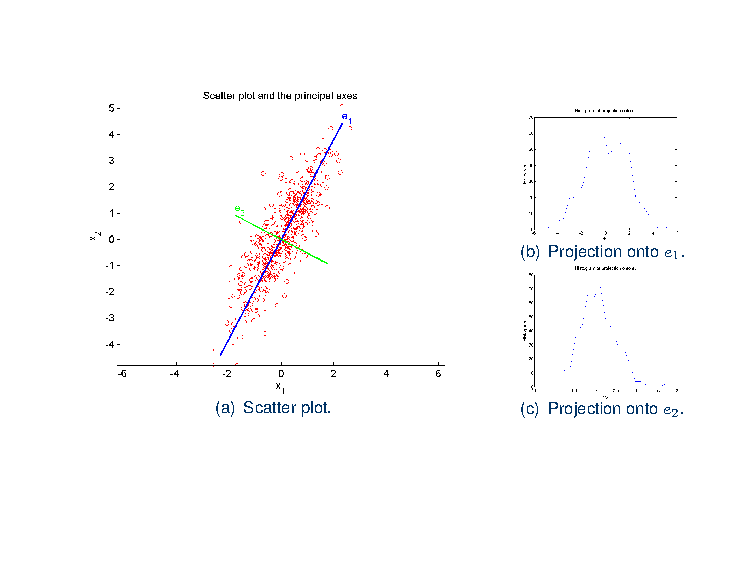
\includegraphics[scale=0.95]{PCA03}
\caption{Scatter plot (red dots) and the principal axes for a bivariate sample. The blue line shows the axis ${\rm e}_1$ with the greatest variance and the green line shows the axis ${\rm e}_2$ with the smallest variance. Features are now uncorrelated.}
\end{figure}
\end{frame}

\begin{frame}{Examples}
\begin{figure}
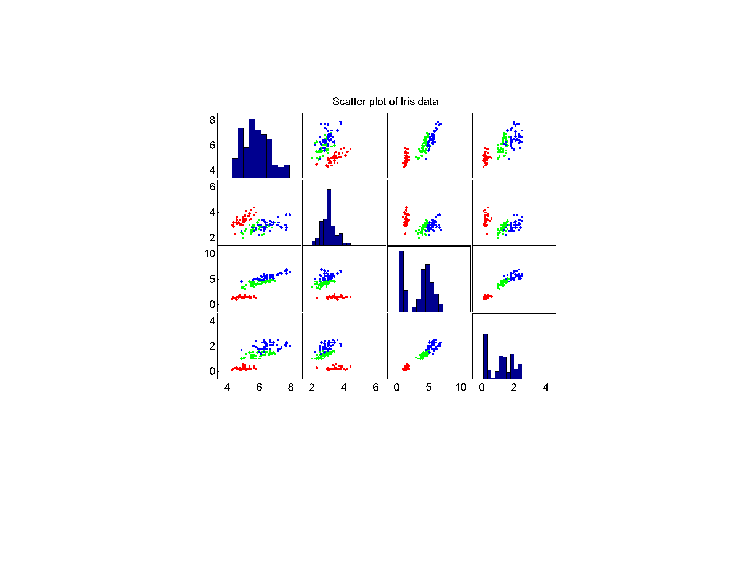
\includegraphics[scale=1]{PCA02}
\caption{Scatter plot of the iris data. Diagonal cells show the histogram for each feature. Other cells show scatters of pairs of features $x_1, x_2, x_3, x_4$ in
top-down and left-right order. Red, green and blue points represent samples for the setosa, versicolor and virginica classes, respectively.}
\end{figure}
\end{frame}

\begin{frame}{Example}
\begin{figure}
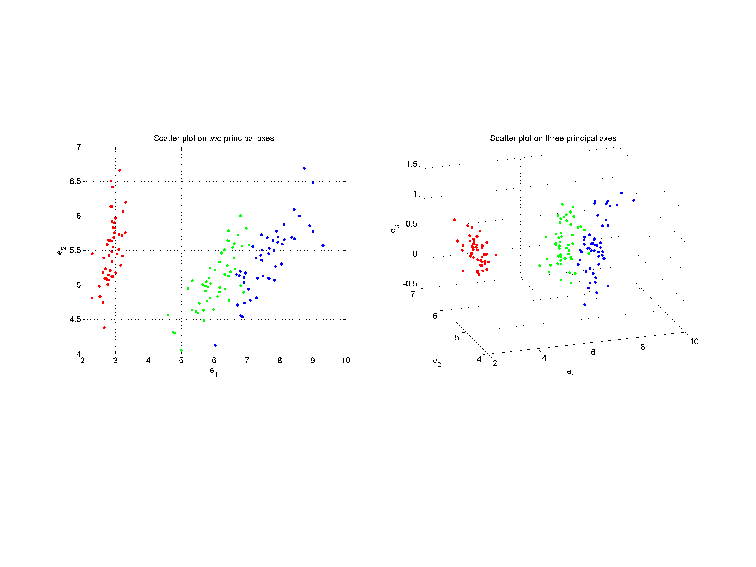
\includegraphics[scale=1]{PCA01}
\caption{Scatter plot of the projection of the iris data onto the first two and the first three principal axes. Red, green and blue points represent samples for the setosa, versicolor and virginica classes, respectively.}
\end{figure}
\end{frame}

\section[LDA]{Linear Discriminant Analysis}
\subsection{}

\begin{frame}{}
\begin{variableblock}{\centering \Large \textbf{\vspace{4pt}\newline Linear Discriminant Analysis\vspace{4pt}}}{bg=slidecolor,fg=white}{bg=slidecolor,fg=white}
\end{variableblock}
\end{frame}

%\begin{frame}{Linear Discriminant Analysis}
%\begin{itemize}
%\item Fisher's linear discriminant
%\begin{itemize}
%\item preserve class separation (special case of principle component analysis)
%\end{itemize}
%\item Multi-dimensional scaling
%\begin{itemize}
%\item Preserve distance measures
%\end{itemize}
%\item Principal component analysis
%\begin{itemize}
%\item Best data representation (not necessarily best class separation)
%\end{itemize}
%\end{itemize}
%\end{frame}

\begin{frame}{Fisher Linear Discriminant}
\begin{itemize}
\item PCA seeks directions that are efficient for
representation, \textit{\color{mycolor2}discriminant analysis} seeks directions that are efficient for discrimination.
\item Suppose ${\rm x}_1,{\rm x}_2,\ldots,{\rm x}_n\in \mathbb{R}^d$ are divided into two subsets $\mathcal{D}_1$ ($n_1$  samples) and $\mathcal{D}_2$ ($n_2$  samples)
corresponding to the classes $\omega_1$ and $\omega_2$ respectively, the
goal is to find a projection onto a line defined as
\begin{equation}
{y}={\rm w}^T{\rm x} \nonumber
\end{equation}
where the points corresponding to $\mathcal{D}_1$ and $\mathcal{D}_2$ are well separated.
\item A corresponding set of $n$ samples ${y}_1,{y}_2,\ldots,{y}_n$ divided into the subset $\mathcal{Y}_1$ and $\mathcal{Y}_2$.\nocite{duda2012pattern}
\end{itemize}
\end{frame}

%\begin{frame}{Fisher's linear discriminant (2-class)}
%\begin{itemize}
%\item Given $n$ $d$-dimensional samples ${\rm x}_1,{\rm x}_2,\ldots,{\rm x}_n$,
%\begin{itemize}
%\item subset $\mathcal{D}_1$ labeled $\omega_1,~n_1$
%\item subset $\mathcal{D}_2$ labeled $\omega_2,~n_2$
%\item $n_1+n_2 = n$
%\end{itemize}
%\item Linear combination of the components
%\begin{equation}
%{\rm y} = {\rm w}^T{\rm x} \nonumber
%\end{equation}
%which maps d-dimensional samples on line, best preserves class separation
%\item Intuitively, good features are those with large separation of means relative to variances.
%\end{itemize}
%\end{frame}

\begin{frame}{Fisher Linear Discriminant}
\begin{figure}
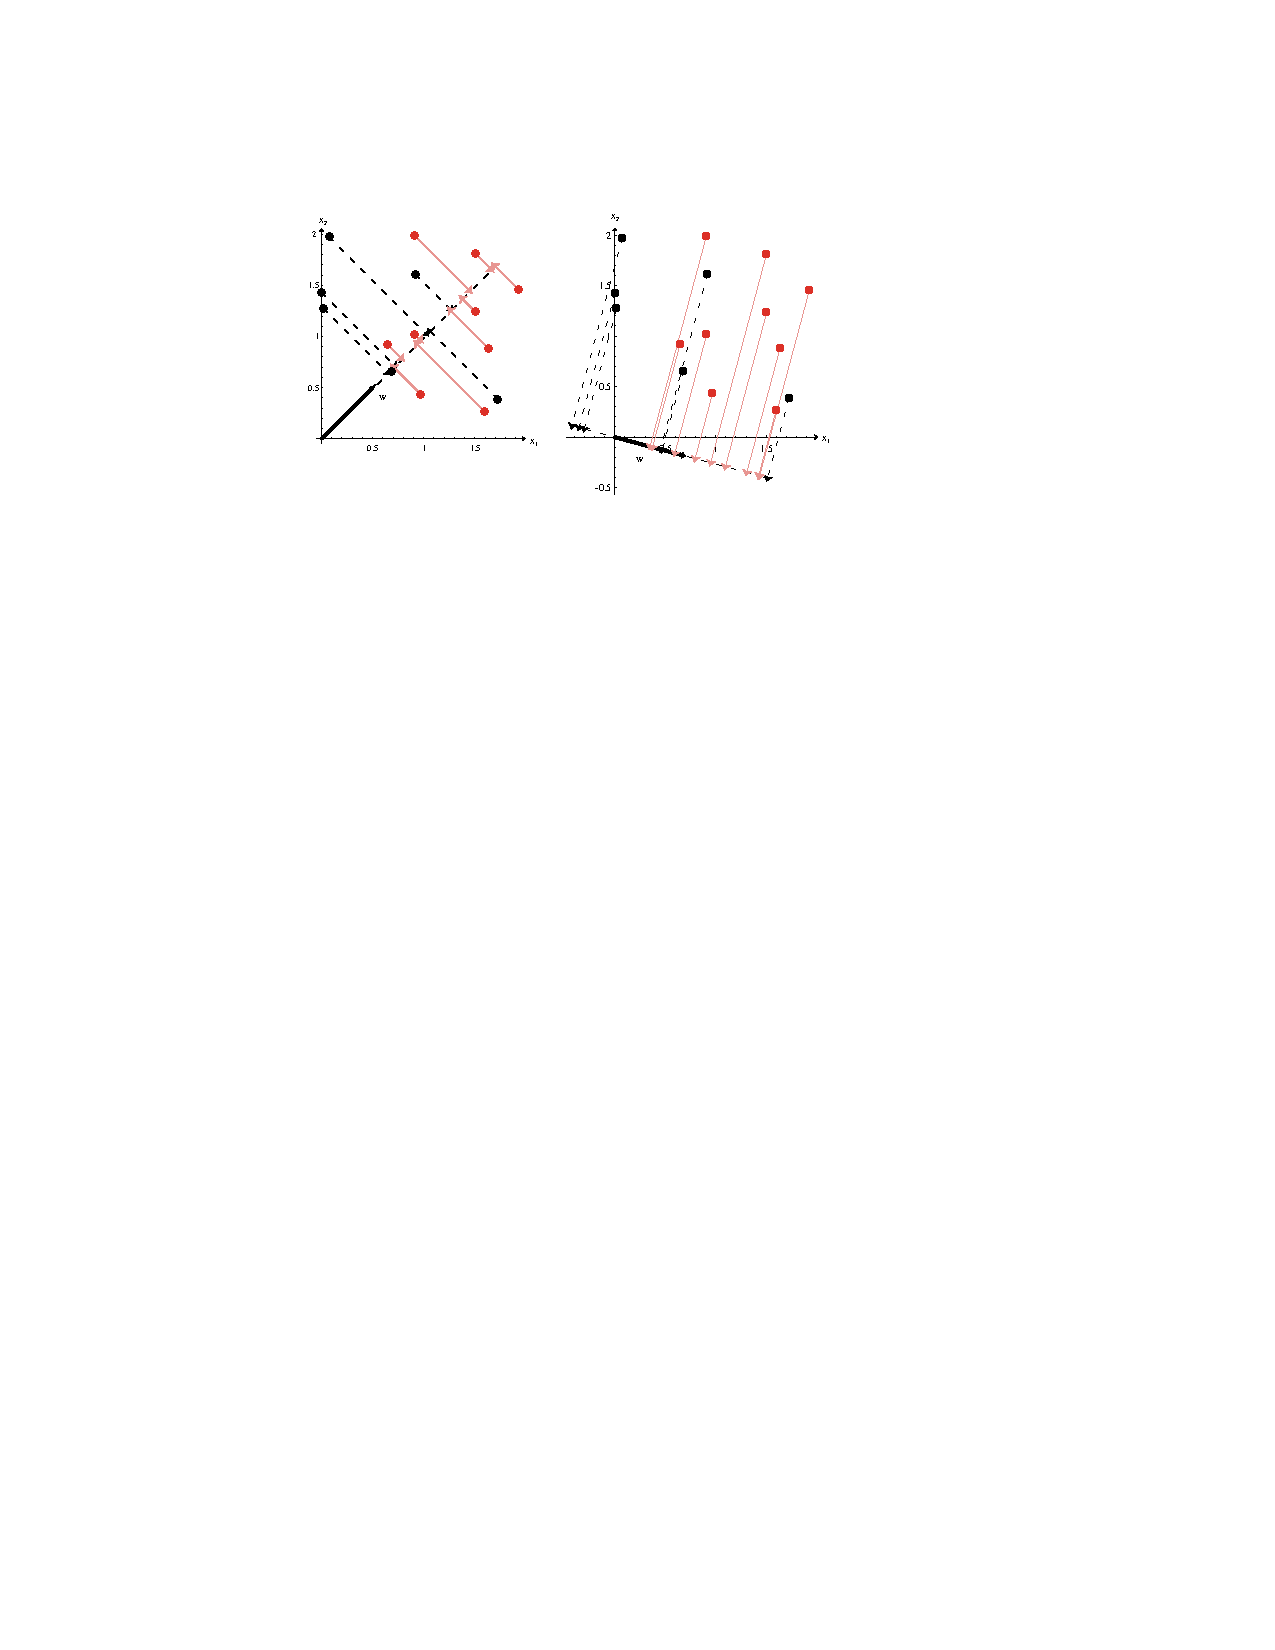
\includegraphics[scale=1.1]{Fisher01}
\caption{Projection of the same set of samples onto two different lines in the directions marked as ${\rm w}$. The figure on the right shows greater separation between the red and black projected points}
\end{figure}
\end{frame}

\begin{frame}{Fisher Linear Discriminant}
\begin{itemize}
\item The criterion function for the best separation can be defined as
\begin{figure}

\includegraphics[scale=1]{LDA01}
\end{figure}
where, $\tilde{m}_i$ is the sample mean and $\tilde{s}_i^2$ is the scatter for the projected samples labeled $\omega_i$, given as
\begin{figure}

\includegraphics[scale=0.9]{LDA03}~~~~~~~~
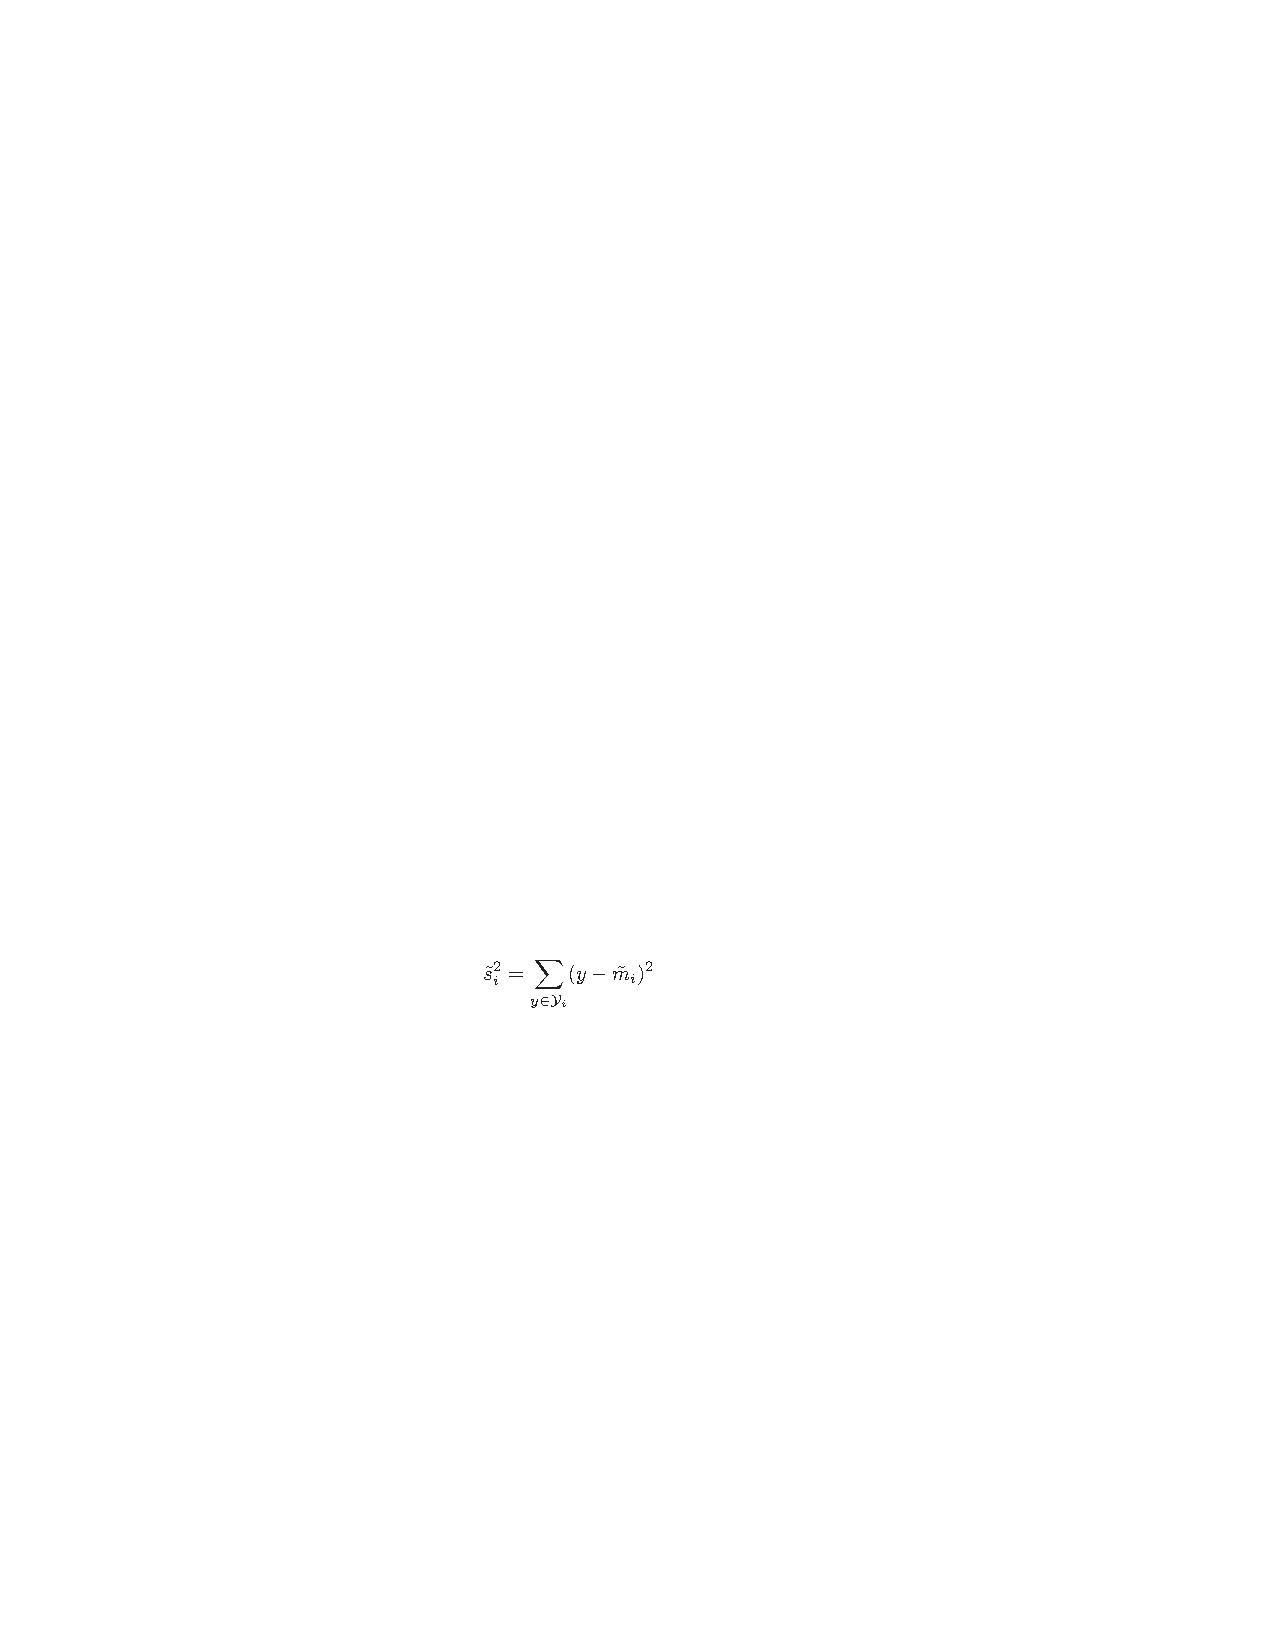
\includegraphics[scale=0.9]{LDA02}
\end{figure}
\item This is called the \textit{\color{mycolor2}Fisher's linear discriminant} with the
geometric interpretation that the best projection makes the
difference between the means as large as possible relative
to the variance.
\end{itemize}
\end{frame}

\begin{frame}{Fisher Linear Discriminant}
\begin{itemize}
\item To compute the optimal ${\rm w}$, we define the \textit{\color{mycolor2}scatter matrices} ${\rm S}_i$
\begin{figure}

\includegraphics[scale=1]{LDA04}
\end{figure}
where,
\begin{figure}
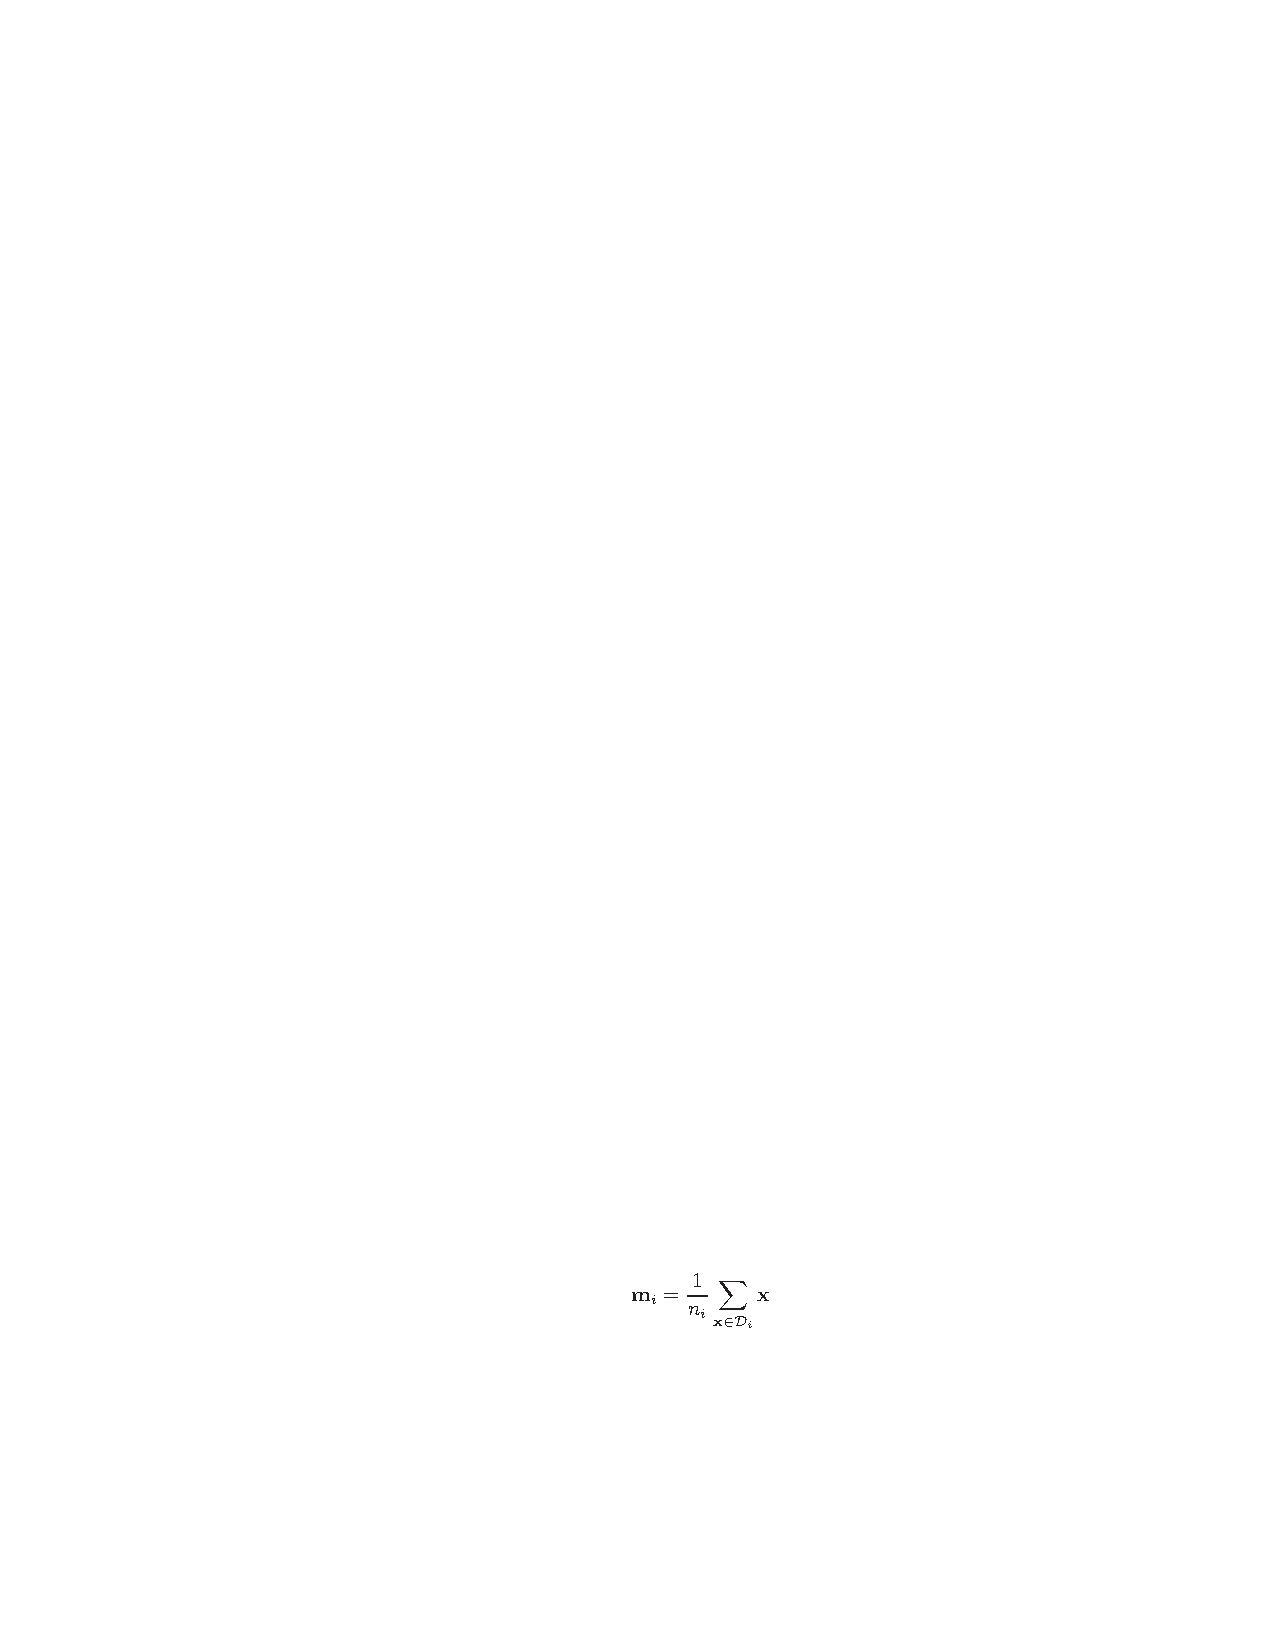
\includegraphics[scale=1]{LDA05}
\end{figure}
\item The \textit{\color{mycolor2}within-class scatter matrix} ${\rm S_ W}$
\begin{figure}

\includegraphics[scale=1]{LDA06}
\end{figure}
and the \textit{\color{mycolor2}between-class scatter matrix} ${\rm S_B}$
\begin{figure}

\includegraphics[scale=1]{LDA07}
\end{figure}
\end{itemize}
\end{frame}

\begin{frame}{Fisher Linear Discriminant}
\begin{itemize}
\item Then, the criterion function becomes
\begin{figure}

\includegraphics[scale=1]{LDA08}
\end{figure}
This expression is well known in mathematical physics as the generalized Rayleigh quotient.
\item A vector ${\rm w}$ that maximizes $J(\cdot)$ must satisfy
\begin{align}
{\rm S}_B{\rm w}&=\lambda {\rm S}_W{\rm w} \nonumber\\
{{\rm S}_W}^{-1}{\rm S}_B{\rm w}&=\lambda {\rm w}\nonumber
\end{align}
\item In this perticular case, it is unnecessary to solve for the eigenvalues and eigenvectors of ${{\rm S}_W}^{-1}{\rm S}_B$ due to the fact that ${\rm S}_B{\rm w}$ is always in the direction of ${\rm m}_1-{\rm m}_2$
\end{itemize}
\end{frame}

\begin{frame}{Fisher Linear Discriminant}
\begin{itemize}
\item So we can find the immediate solution as
\begin{figure}

\includegraphics[scale=1]{LDA09}
\end{figure}
\item Note that, ${\rm S_W}$ is symmetric and positive semidefinite, and it is usually nonsingular if $n > d$. ${\rm S_B}$ is also symmetric and positive semidefinite, but its rank is at most 1.
\item Thus, we have obtained ${\rm w}$ for Fisher's linear discriminant -- the linear function yielding the maximum ratio of between-class scatter to within-class scatter.
\end{itemize}
\end{frame}

\begin{frame}{Multiple Discriminant Analysis}
\begin{itemize}
\item For the $c$-class problem
\item The natural generalization of Fisher's linear discriminant involves $c-1$ discriminant functions.

\item Thus, the projection is from a $d$-dimensional space to a $(c-1)$-dimensional space, and it is assumed that $d\geq c$.
\item The criteria function is
\begin{figure}
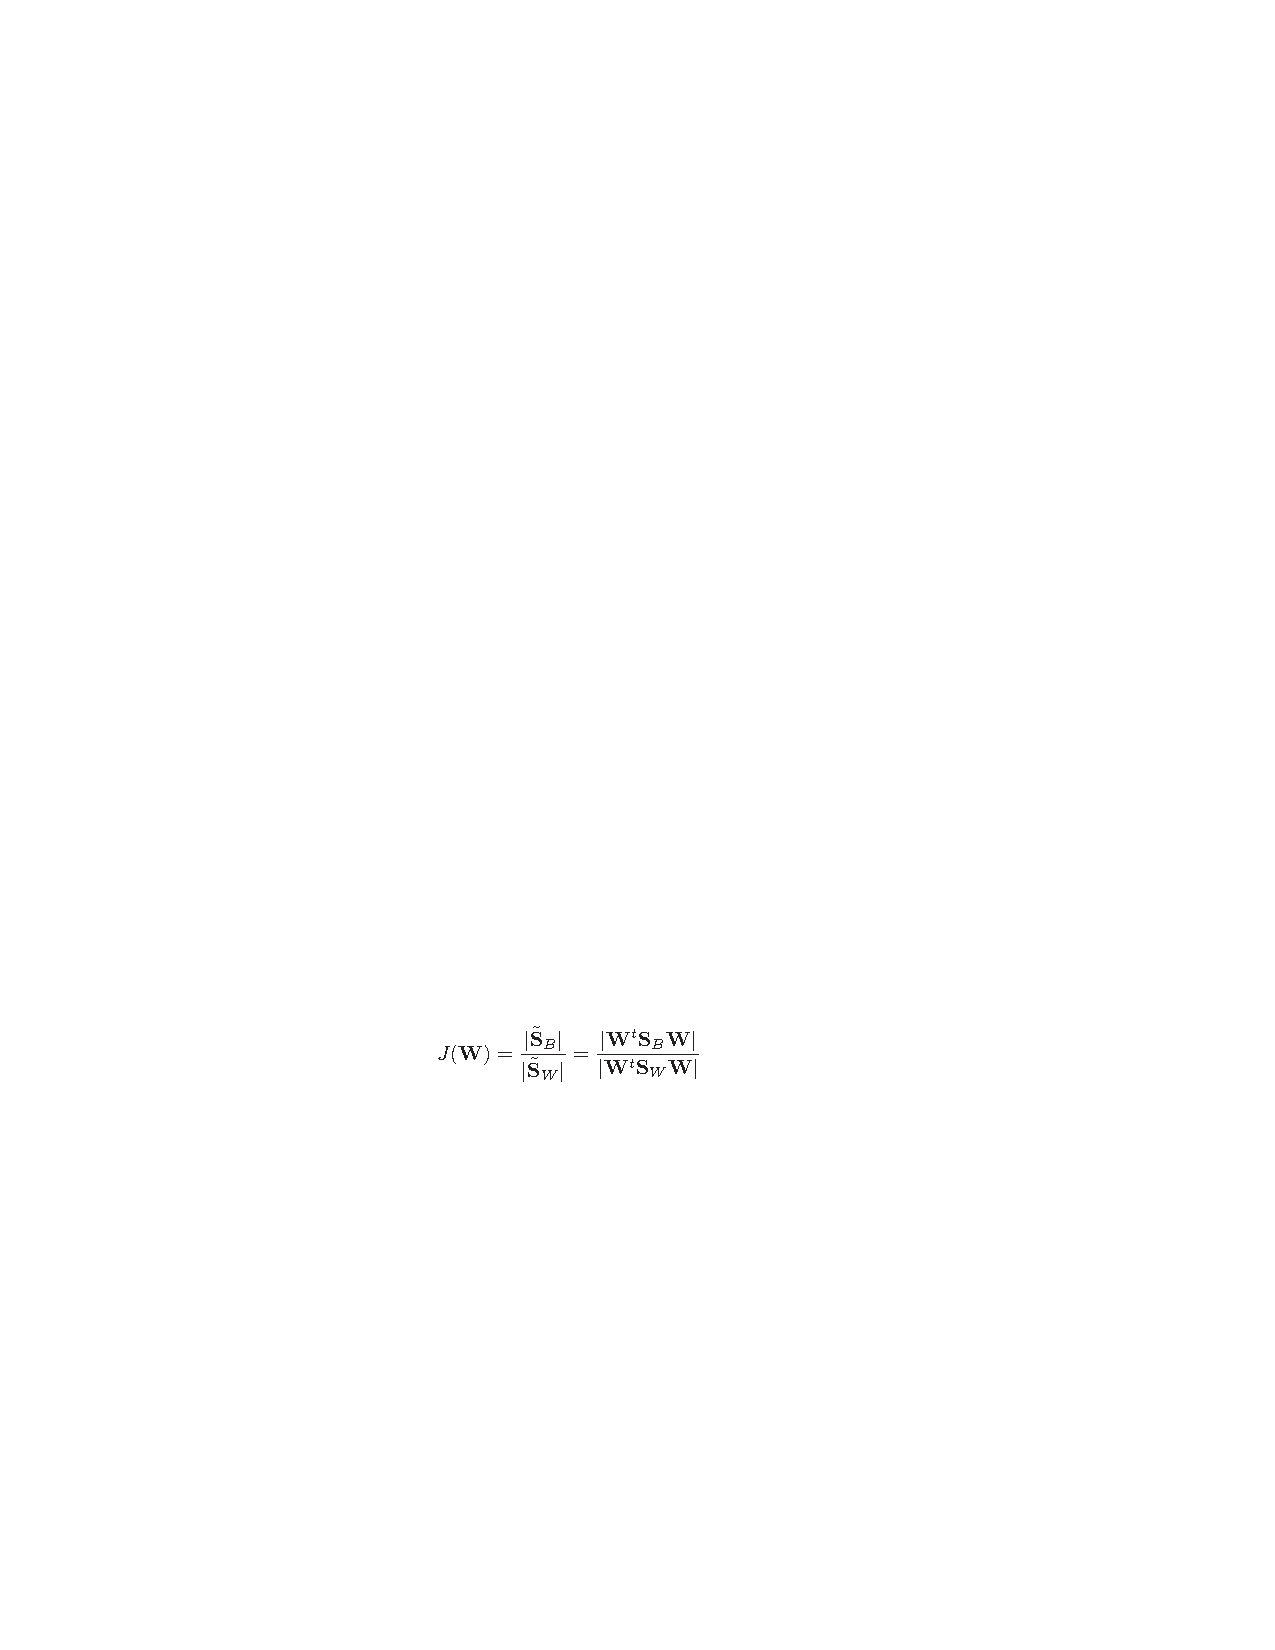
\includegraphics[scale=1]{ldf07}
\end{figure}
The problem of finding a rectangular matrix ${\rm W}$ that maximizes $J(\cdot)$
\end{itemize}
\end{frame}

\begin{frame}{Multiple Discriminant Analysis}
\begin{itemize}
\item The within-class scatter matrix
\begin{figure}

\includegraphics[scale=1]{ldf08}
\end{figure}
where\\
\begin{figure}

\includegraphics[scale=1]{ldf09}~~~~~~
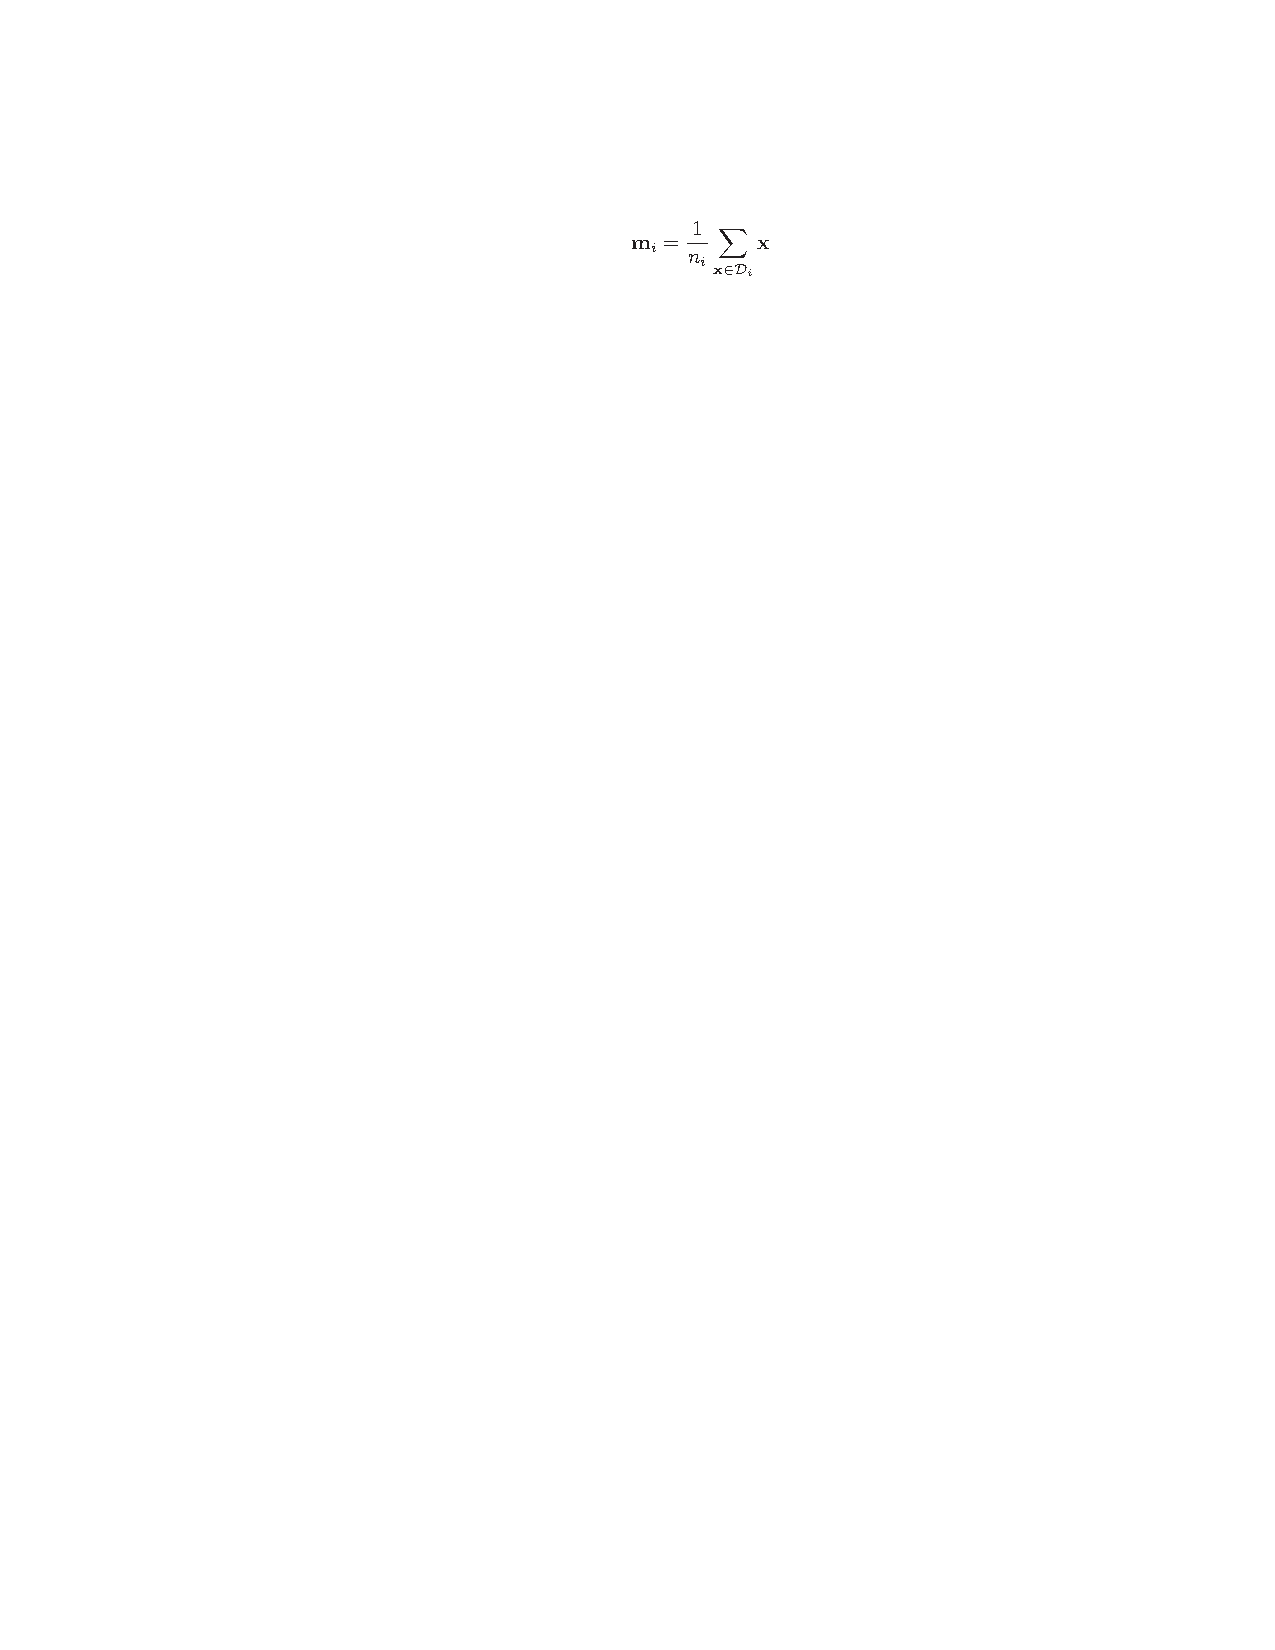
\includegraphics[scale=1]{ldf10}
\end{figure}
\item The proper generalization for ${\rm S}_B$ is not quite so obvious.
\item Suppose that we define a \textit{\color{mycolor2}total mean vector} ${\rm m}$ and a total scatter matrix ${\rm S}_T$ by
\begin{figure}
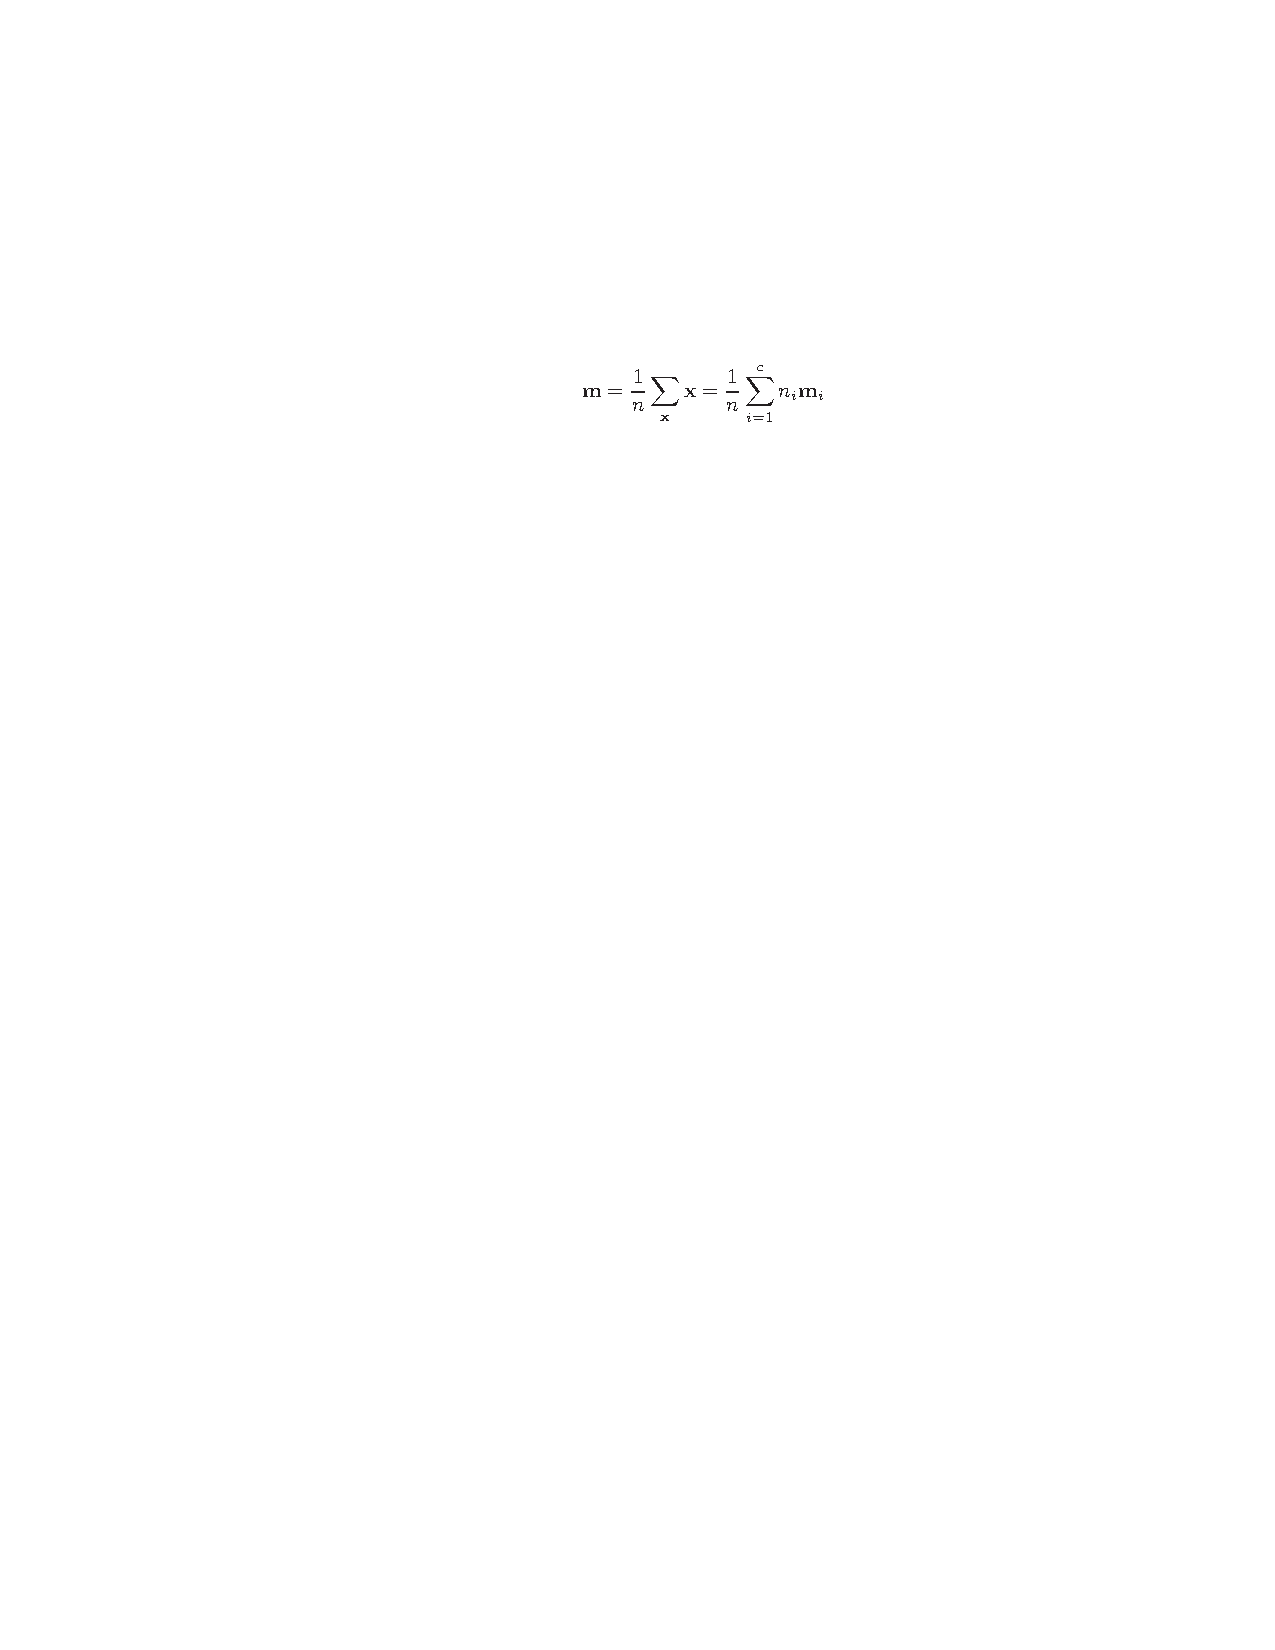
\includegraphics[scale=1]{ldf11}~~~~~~~
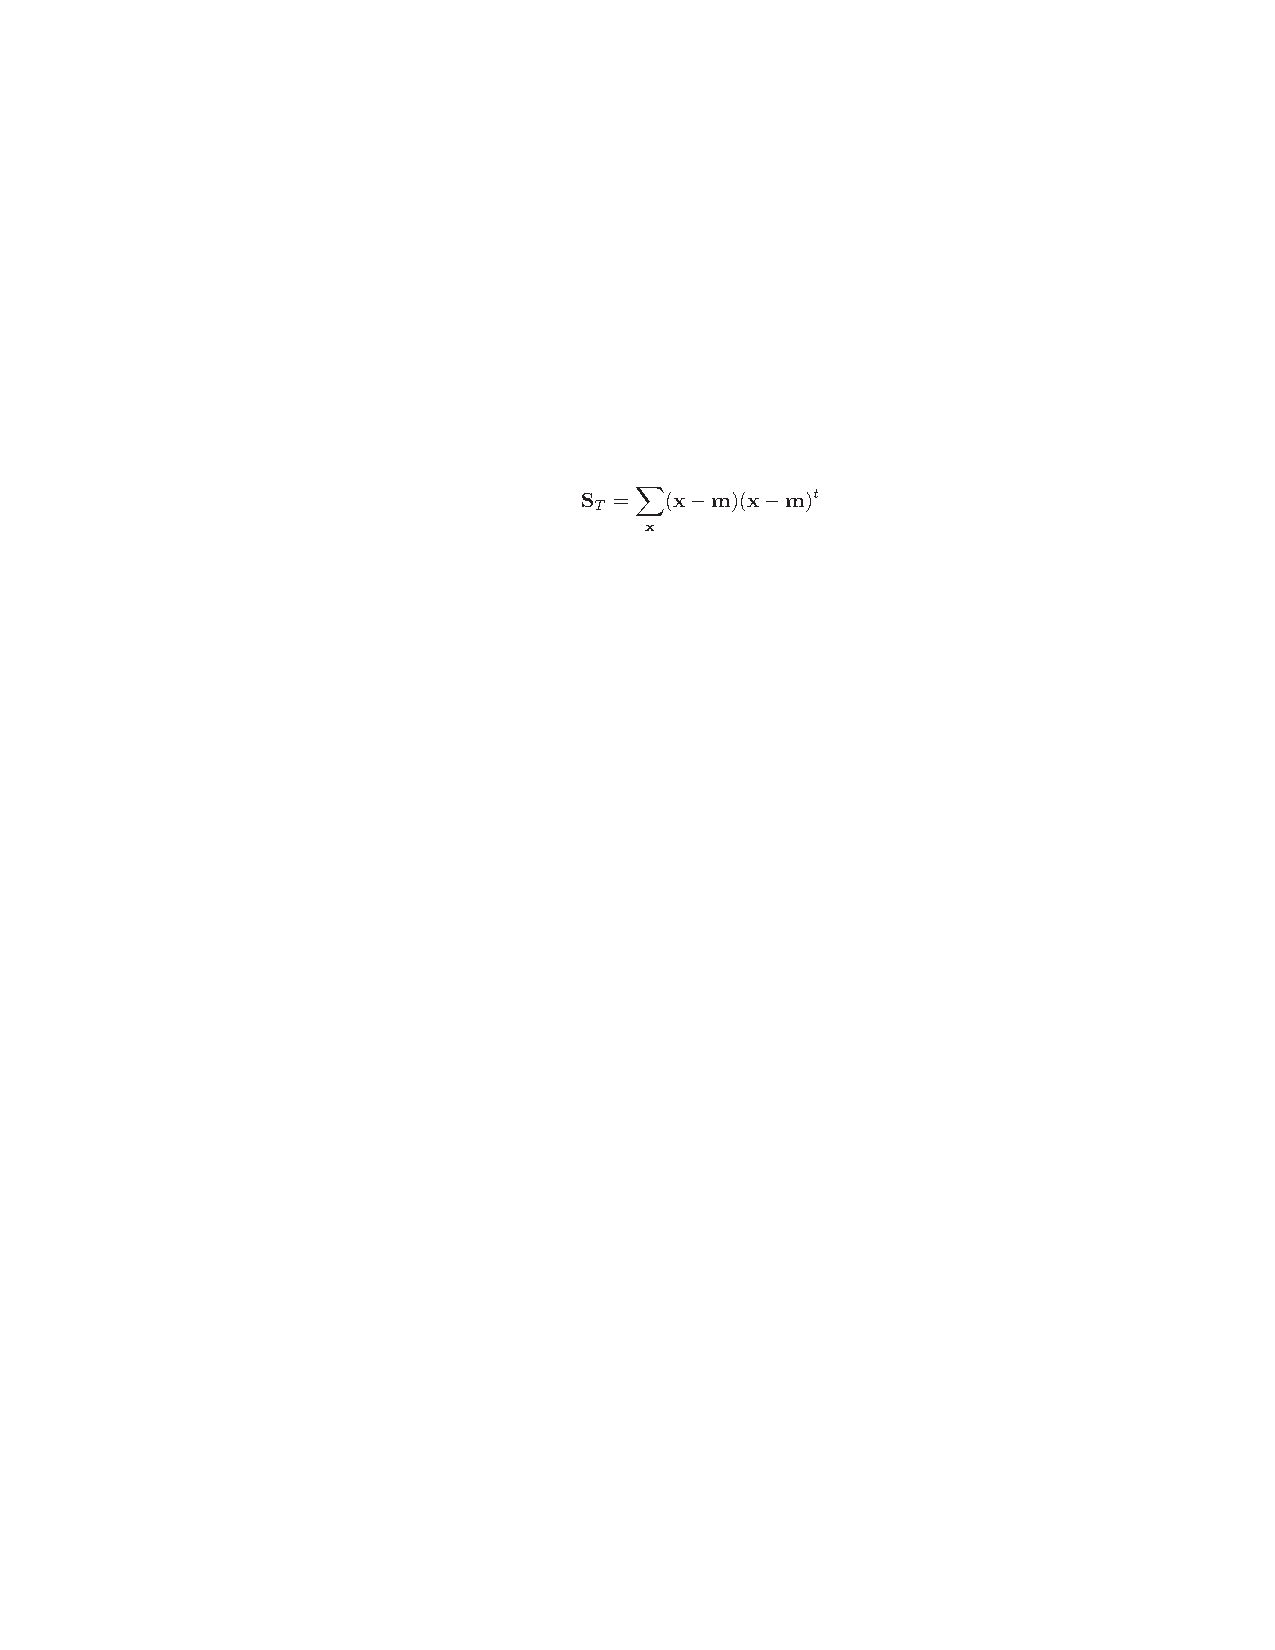
\includegraphics[scale=1]{ldf12}
\end{figure}
\end{itemize}
\end{frame}

\begin{frame}{Multiple Discriminant Analysis}
\begin{itemize}
\item Then we can write
\begin{figure}
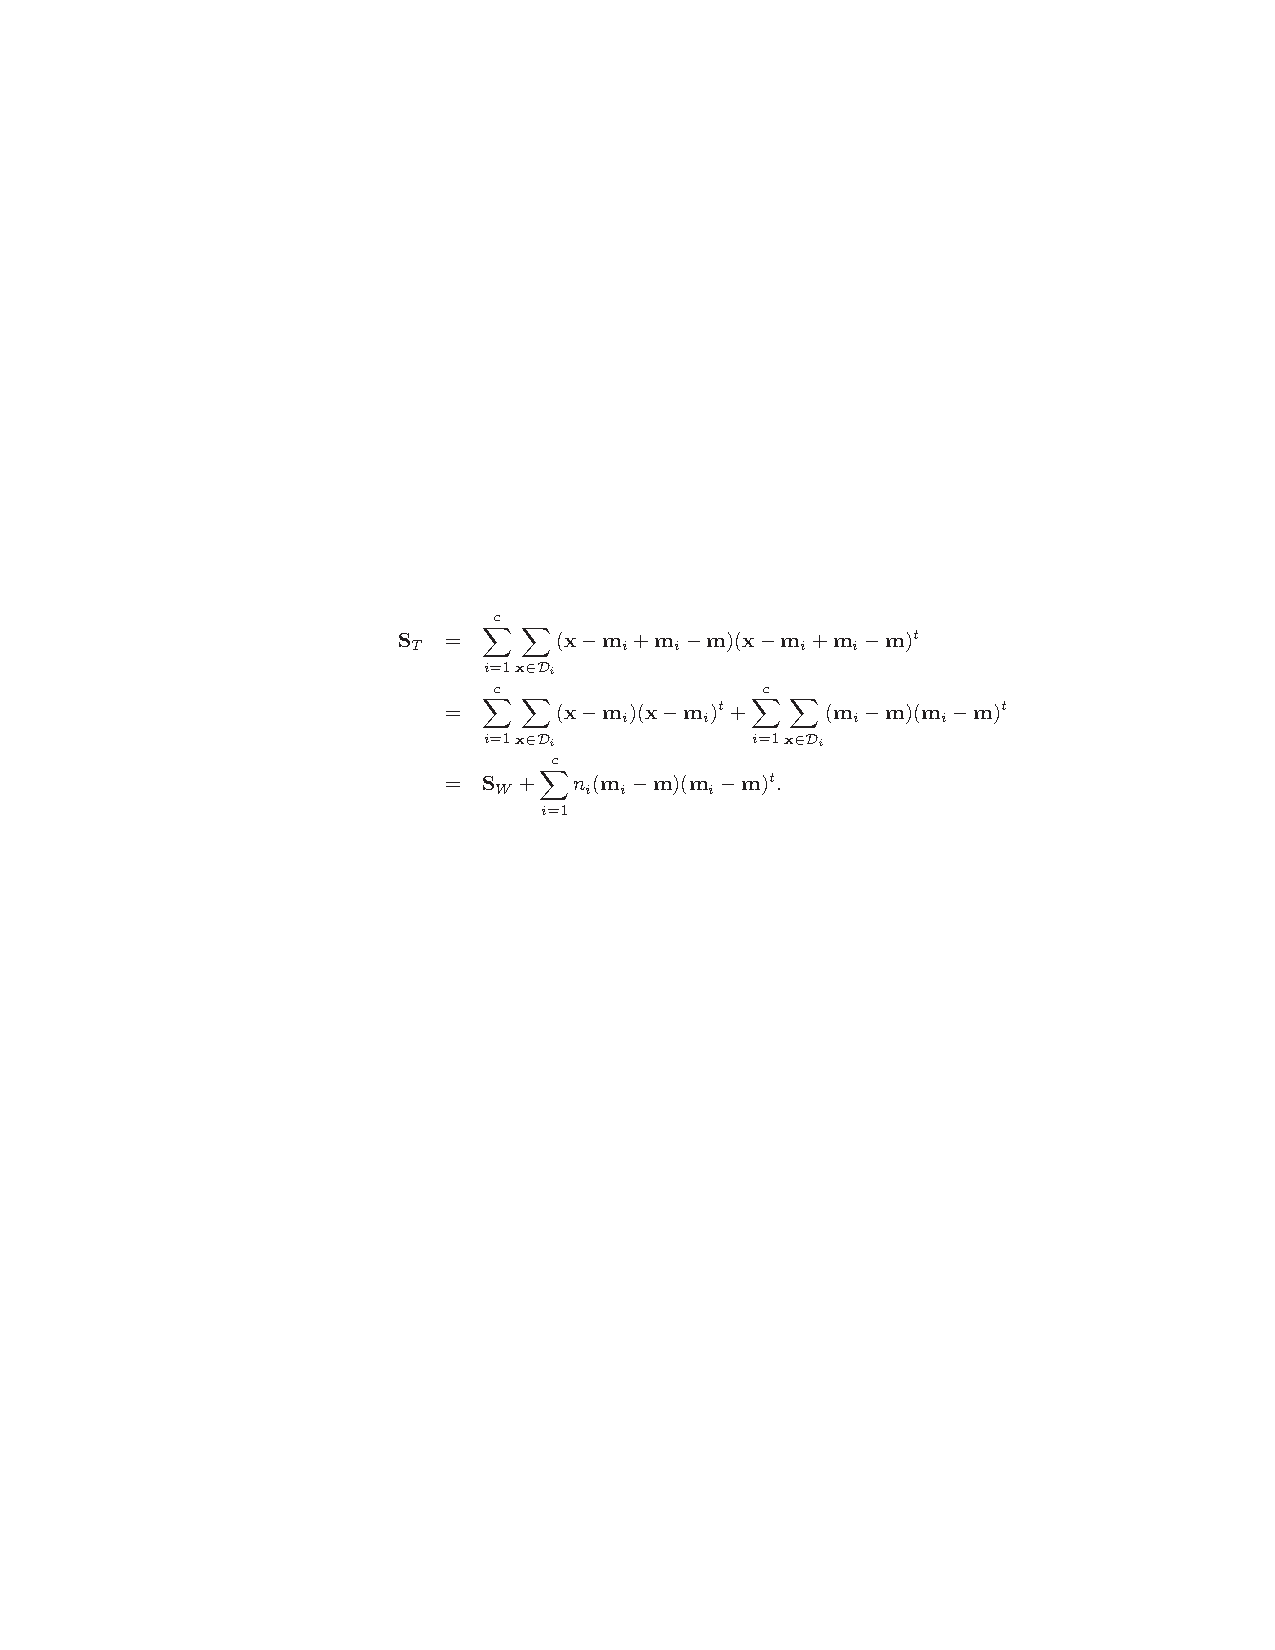
\includegraphics[scale=0.9]{ldf13}
\end{figure}
\item Therefore,
\begin{equation}
{\rm S}_T={\rm S}_{W}+{\rm S}_{B}\nonumber
\end{equation}
where 
\begin{figure}

\includegraphics[scale=0.9]{ldf14}
\end{figure}
\end{itemize}
\end{frame}

\begin{frame}{Multiple Discriminant Analysis}
\begin{itemize}
\item The projection form a $d$-dimensional space to a $(c-1)$-dimensional space is accomplished by $c-1$ discriminant functions
\begin{figure}

\includegraphics[scale=1]{ldf15}
\end{figure}
\item If the $y_i$ are viewed as components of a vector ${\rm y}$ and the weight vector ${\rm w}_i$ are viewed as the columns of a $d$-by-$(c-1)$ matrix ${\rm W}$, then the projection can be written as a single matrix equation
\begin{figure}

\includegraphics[scale=1]{ldf16}
\end{figure}
\end{itemize}
\end{frame}

\begin{frame}{Multiple Discriminant Analysis}
\begin{itemize}
\item The samples ${\rm x}_1,{\rm x}_2,\ldots,{\rm x}_n$ project to a corresponding set of samples ${\rm y}_1,{\rm y}_2,\ldots,{\rm y}_n$, which can be described by their own mean vectors and scatter matrices. Thus
\begin{figure}
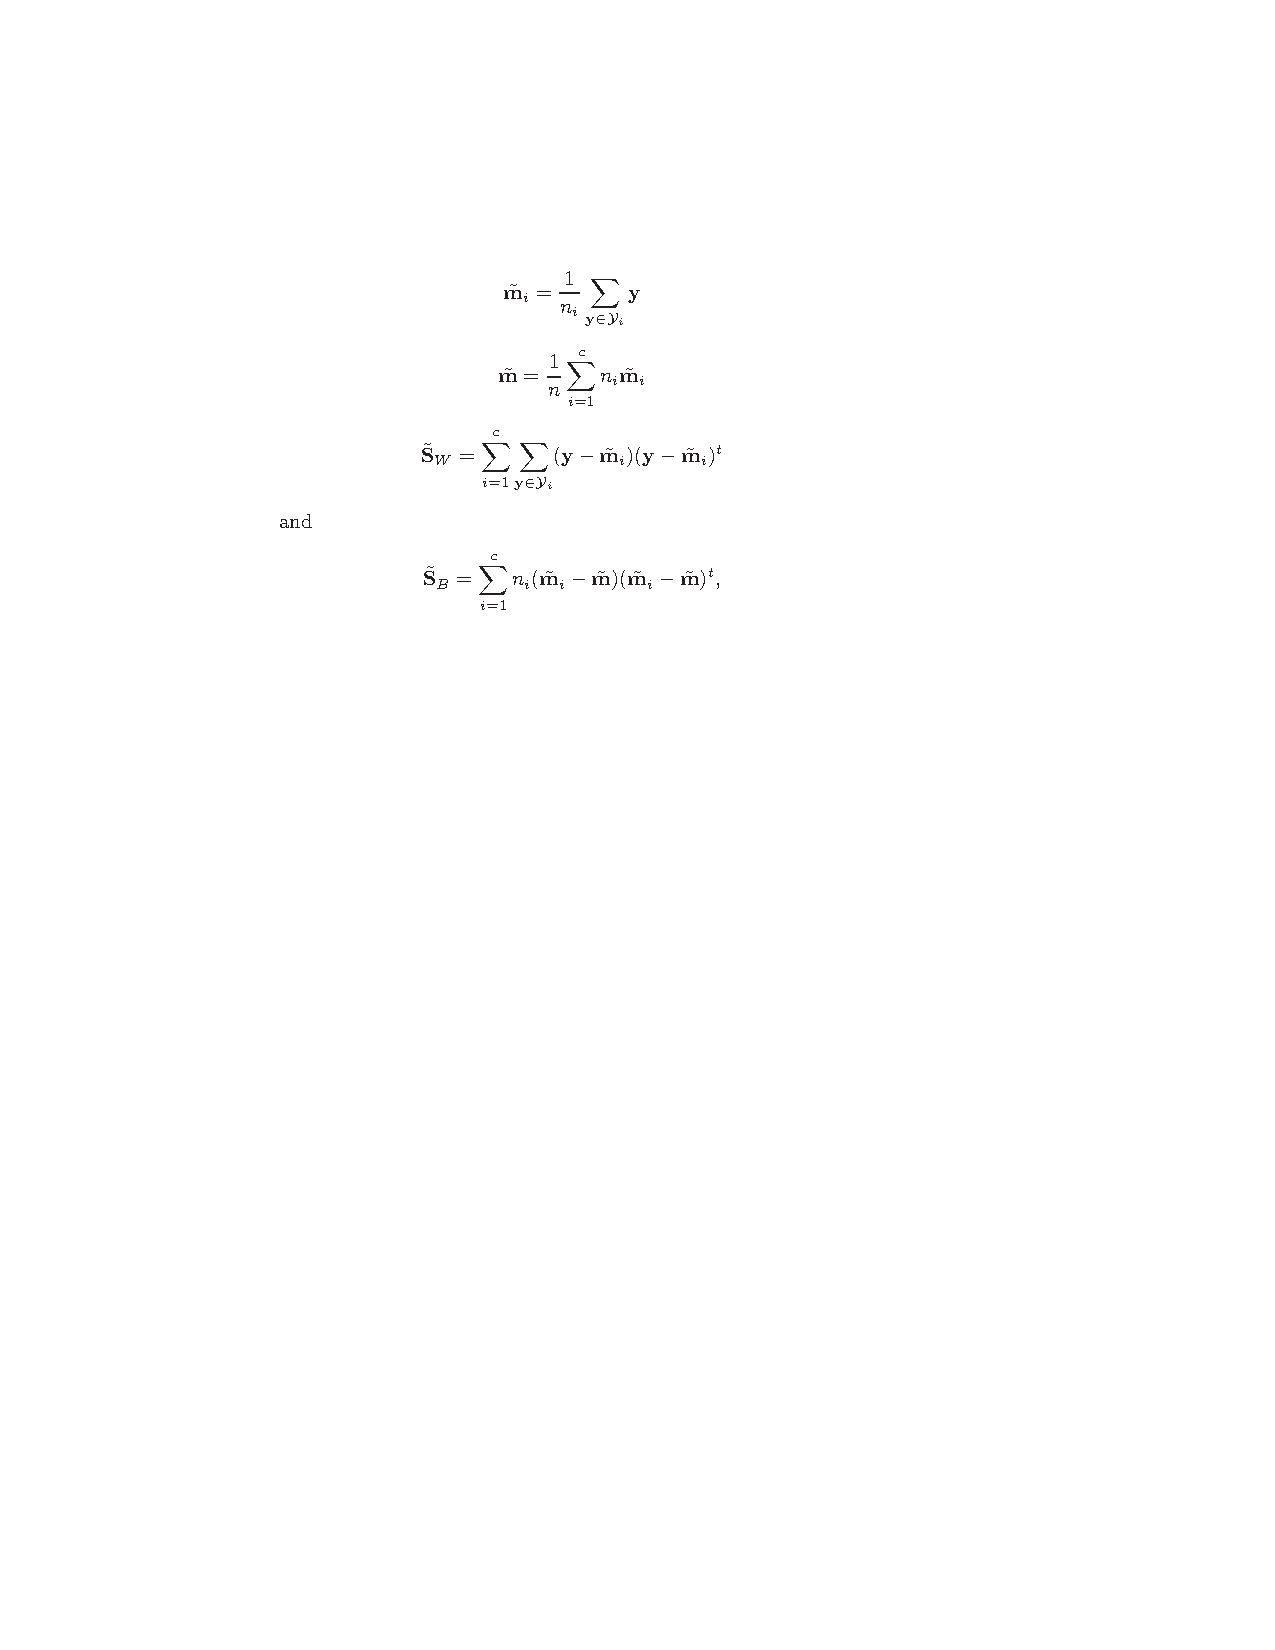
\includegraphics[scale=0.9]{ldf18}
\end{figure}
\end{itemize}
\end{frame}

\begin{frame}{Multiple Discriminant Analysis}
\begin{itemize}
\item It is a straightforward matter to show that
\begin{figure}

\includegraphics[scale=1]{ldf17}
\end{figure}
\item These equations show how the within-class and between-class scatter matrices are transformed by the projection to the lower dimensional space.
\end{itemize}
\end{frame}

\begin{frame}{Multiple Discriminant Analysis}
\begin{figure}
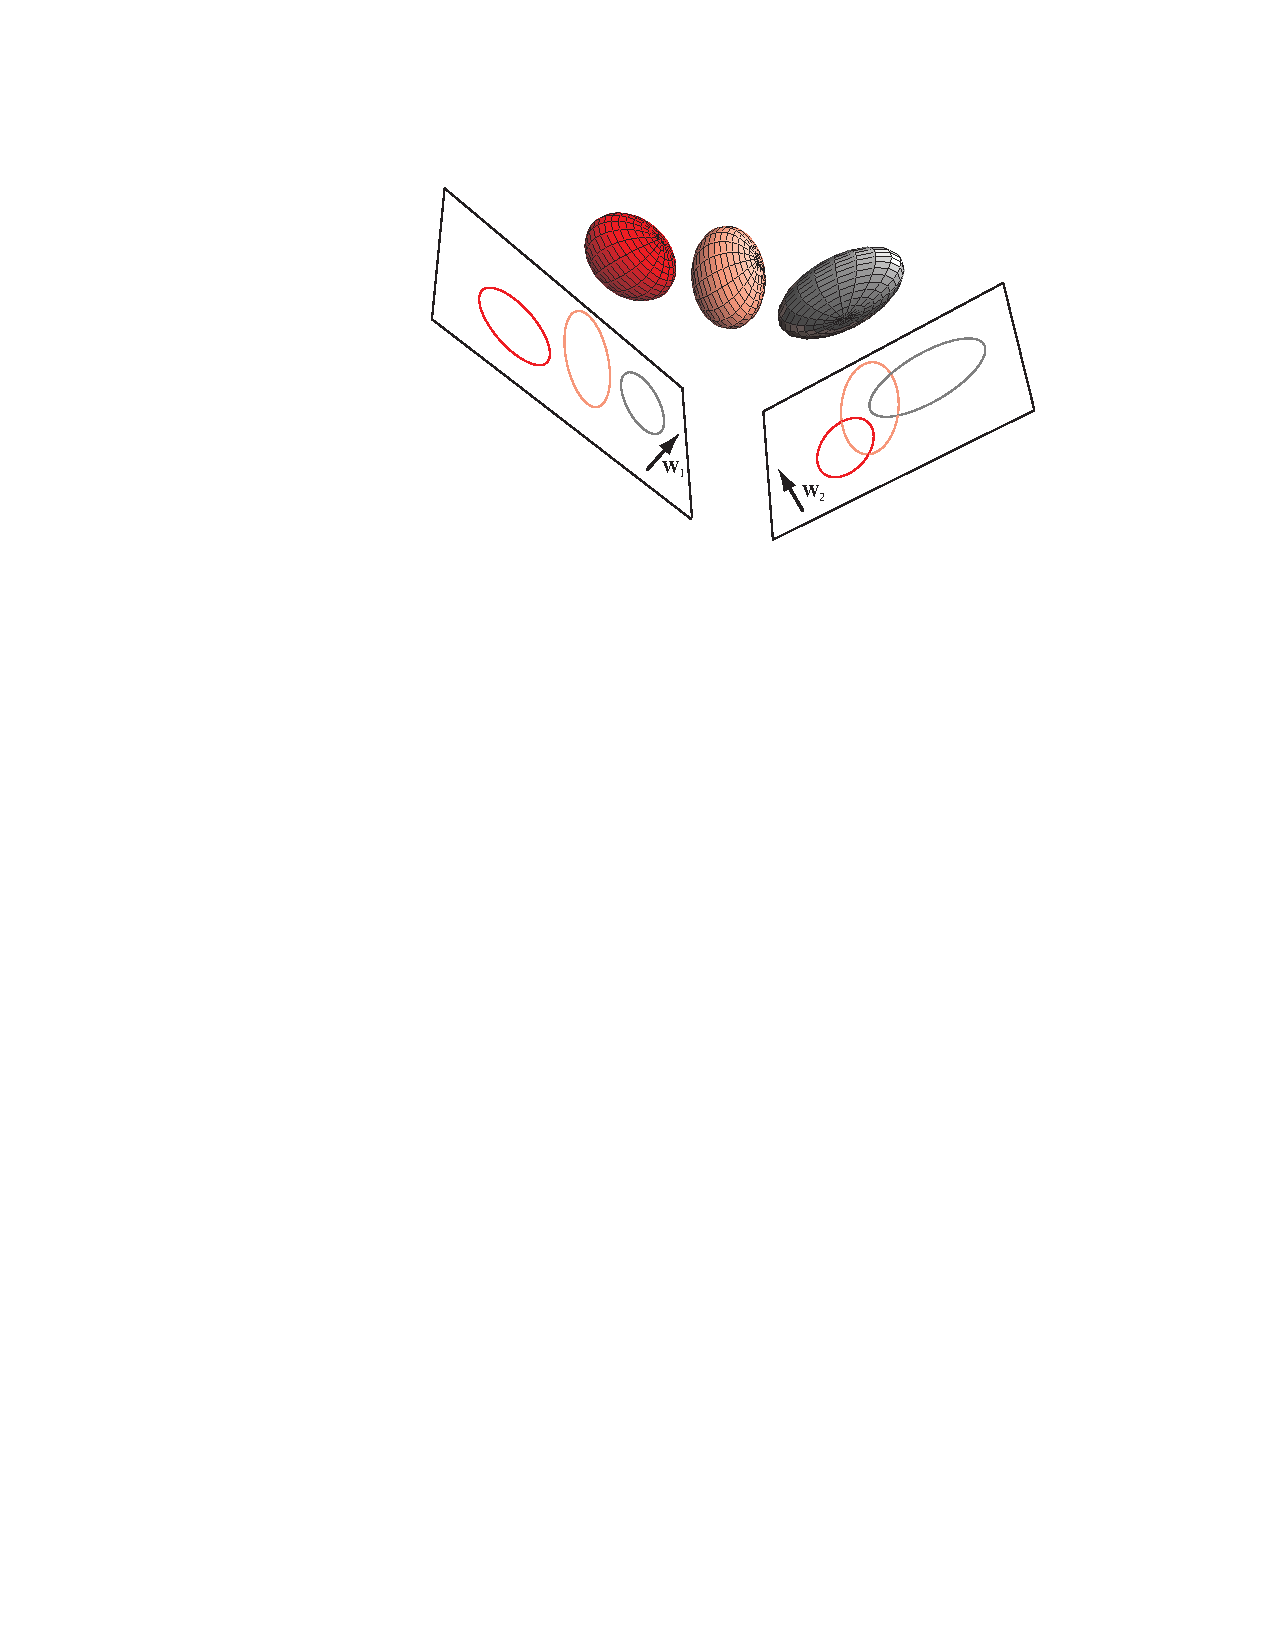
\includegraphics[scale=0.8]{ldf19}
\caption{Three three-dimensional distributions are projected onto two-dimensional
subspaces, described by a normal vectors ${\rm W}_1$ and ${\rm W}_2$ . Informally, multiple discriminant methods seek the optimum such subspace, i.e., the one with the greatest separation of the projected distributions for a given total within-scatter matrix, here as
associated with ${\rm W}_1$}
\end{figure}
\end{frame}

\begin{frame}{Multiple Discriminant Analysis: Solution}
\begin{itemize}
\item The criterion function
\begin{figure}
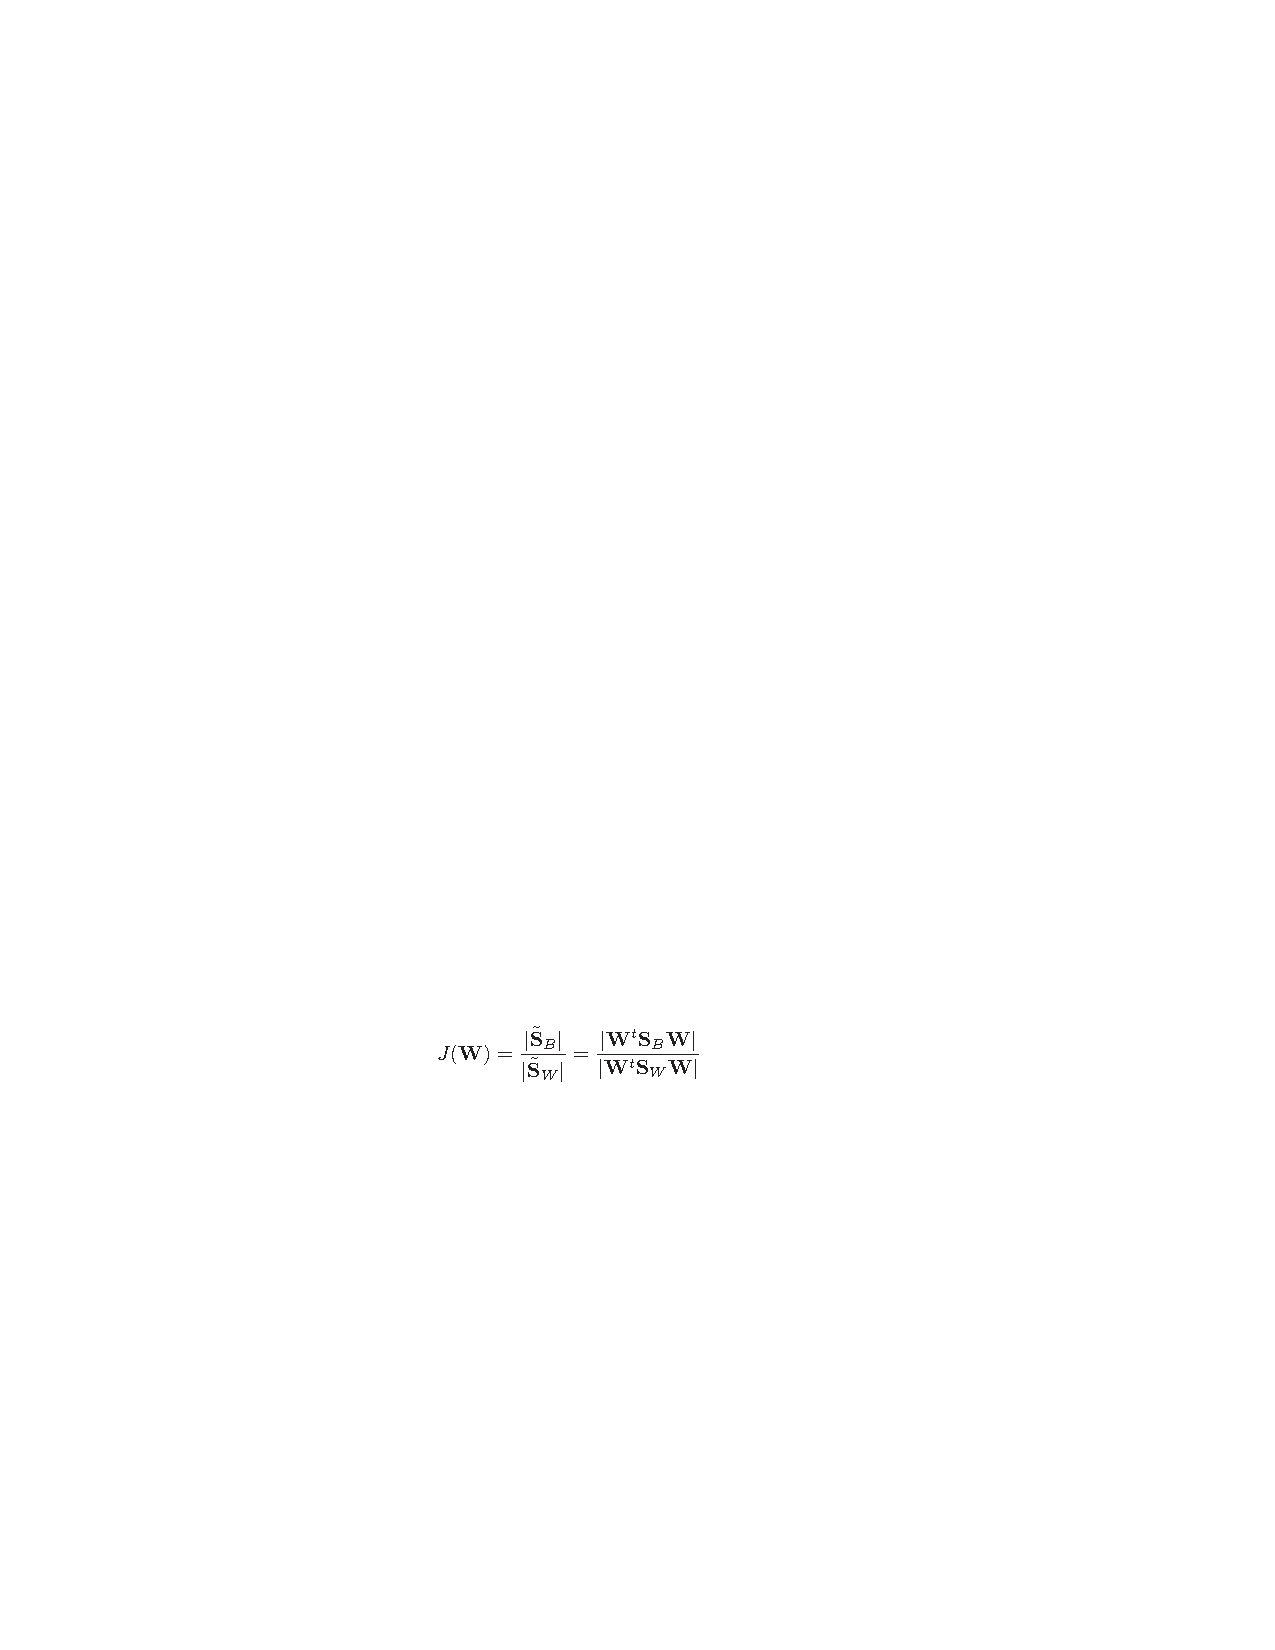
\includegraphics[scale=1]{ldf07}
\end{figure}
the problem of finding a rectangular matrix ${\rm W}$ that maximized $J(\cdot)$. 
\item The columns of an optimal ${\rm W}$ are the generalized eigenvectors that correspond to the largest eigenvalues in
\begin{figure}

\includegraphics[scale=1]{ldf20}
\end{figure}
\end{itemize}
\end{frame}

\begin{frame}{Multiple Discriminant Analysis: Observation}

\begin{figure}

\includegraphics[scale=1]{ldf20}
\end{figure}
\begin{itemize}
\item If ${\rm S}_W$ is nonsingular, this can be converted to a conventional eigenvalue problem as before. 
\item Computation of the inverse of ${\rm S}_W$ is expensive.
\item Instead, one can find the eigenvalues as the roots of the characteristic polynomial
\begin{figure}

\includegraphics[scale=1]{ldf21}
\end{figure}
\item and then solve
\begin{figure}

\includegraphics[scale=1]{ldf22}
\end{figure}
directly for the eigenvectors ${\rm w}_i.$
\end{itemize}
\end{frame}


\section{Feature Selection}
\subsection{}
\begin{frame}{}
\begin{variableblock}{\centering \Large \textbf{\vspace{4pt}\newline Feature Selection\vspace{4pt}}}{bg=slidecolor,fg=white}{bg=slidecolor,fg=white}
\end{variableblock}
\end{frame}

\begin{frame}{Feature Selection}
\begin{itemize}
\item An alternative to feature reduction that uses linear or
non-linear combinations of features is feature selection that
reduces dimensionality by selecting subsets of existing
features.
\item The first step in feature selection is to define a criterion
function that is often a function of the classification error.
\item Note that, the use of classification error in the criterion function makes feature selection procedures dependent on
the specific classifier used.
\end{itemize}
\end{frame}

\begin{frame}{Feature Selection}
\begin{itemize}
\item The most straightforward approach would require
\begin{itemize}
\item examining all $\left( {\begin{array}{*{20}{c}}
d\\
m
\end{array}} \right)$ possible subsets of size $m$,
\item selecting the subset that performs the best according to the criterion function.
\end{itemize}
\item The number of subsets grows combinatorially, making the
exhaustive search impractical.
\item Iterative procedures are often used but they cannot
guarantee the selection of the optimal subset.
\end{itemize}
\end{frame}

\begin{frame}{Feature Selection}
\begin{itemize}
\item \textit{\color{mycolor2}Sequential forward selection:}
\begin{itemize}
\item First, the best single feature is selected.
\item Then, pairs of features are formed using one of the
remaining features and this best feature, and the best pair is
selected.
\item Next, triplets of features are formed using one of the
remaining features and these two best features, and the best
triplet is selected.
\item This procedure continues until all or a predefined number of features are selected.
\end{itemize}
\end{itemize}
\end{frame}

\begin{frame}{Examples}
\begin{figure}
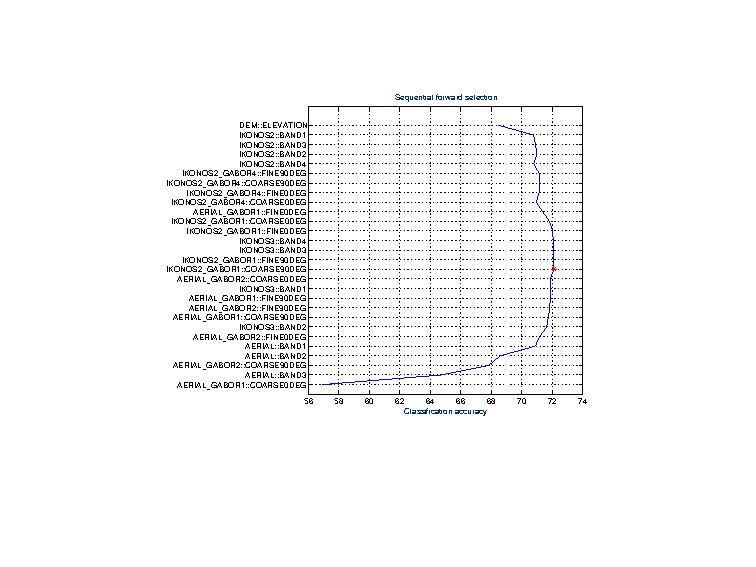
\includegraphics[scale=0.9]{DimProb03}
\caption{Results of sequential forward feature selection for classification of a satellite image using 28 features. $x$-axis shows the classification accuracy (\%) and $y$-axis shows the features added at each iteration (the first iteration is
at the bottom). The highest accuracy value is shown with a star.}
\end{figure}
\end{frame}

\begin{frame}{Feature Selection}
\begin{itemize}
\item \textit{\color{mycolor2}Sequential backward selection:}
\begin{itemize}
\item First, the criterion function is computed for all $d$ features.
\item Then, each feature is deleted one at a time, the criterion
function is computed for all subsets with $d - 1$ features, and
the worst feature is discarded.
\item Next, each feature among the remaining $d - 1$ is deleted one
at a time, and the worst feature is discarded to form a subset
with $d - 2$ features.
\item This procedure continues until one feature or a predefined
number of features are left.
\end{itemize}
\end{itemize}
\end{frame}


\begin{frame}{Examples}
\begin{figure}
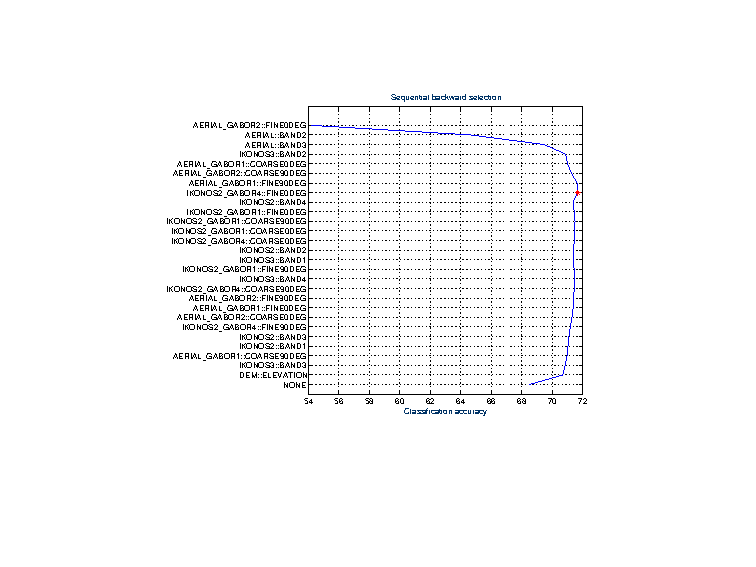
\includegraphics[scale=0.9]{DimProb04}
\caption{Results of sequential backward feature selection for classification of a satellite image using 28 features. $x$-axis shows the classification accuracy (\%) and $y$-axis shows the features removed at each iteration (the first iteration is
at the top). The highest accuracy value is shown with a star.}
\end{figure}
\end{frame}

\begin{frame}{Summary}
\begin{itemize}
\item The choice between feature reduction and feature selection
depends on the application domain and the specific training
data.
\item Feature selection leads to savings in computational costs
and the selected features retain their original physical
interpretation.
\item Feature reduction with transformations may provide a better
discriminative ability but these new features may not have a
clear physical meaning.
\end{itemize}
\end{frame}

\begin{frame}{Problem}
\begin{footnotesize}
\textit{\color{mycolor2}Question:}
\begin{itemize}
\item[(a)] Given the following sets of feature vector belonging to two classes $\omega_1$ and $\omega_2$ which is Gaussian distributed.
\begin{equation}
(1,2)^t,~(3,5)^t,~(4,3)^t,~(5,6)^t, ~(7,5)^t \in \omega_1 \nonumber
\end{equation}
\begin{equation}
(6,2)^t,~(9,4)^t,~(10,1)^t,~(12,3)^t, ~(13,6)^t \in \omega_2 \nonumber
\end{equation}
The vector are projected onto a line to represent the feature vectors by a single feature. Find out the best direction of the line of projection that maintains the separability of the two classes.\\
\item[(b)] Assuming the mean of the projected point belonging to $\omega_1$ to be the origin of the projection line, identify the point on the projection line that optimally separates two two classes. Assume the classes to be equally probable and the projected features also follow Gaussian distribution.
\end{itemize}
\end{footnotesize}
\end{frame}

\section{References}
\subsection{}
\begin{frame}[allowframebreaks]{References}
\linespread{1}
\footnotesize
\printbibliography[heading=none]
\end{frame}
{
\nocite{gose1997pattern}
\setbeamertemplate{logo}{}
\makeatletter
\setbeamertemplate{footline}{
        \leavevmode%
  
  % First line.
  \hbox{%
  \begin{beamercolorbox}[wd=.2\paperwidth,ht=\beamer@decolines@lineup,dp=0pt]{}%
  \end{beamercolorbox}%
  \begin{beamercolorbox}[wd=.8\paperwidth,ht=\beamer@decolines@lineup,dp=0pt]{lineup}%
  \end{beamercolorbox}%
  } %
  % Second line.
  \hbox{%
  \begin{beamercolorbox}[wd=\paperwidth,ht=\beamer@decolines@linemid,dp=0pt]{linemid}%
  \end{beamercolorbox}%
  } %
  % Third line.
  \hbox{%
  \begin{beamercolorbox}[wd=.1\paperwidth,ht=\beamer@decolines@linebottom,dp=0pt]{}%
  \end{beamercolorbox}%
  \begin{beamercolorbox}[wd=.9\paperwidth,ht=\beamer@decolines@linebottom,dp=0pt]{linebottom}%
  \end{beamercolorbox}%
  }%
        }
\makeatother

\begin{frame}
\centering
\includegraphics[width=0.4\paperwidth]{queries.jpg}\\
\includegraphics[width=0.5\paperwidth]{thank_you.png}
\end{frame}
}
